\graphicspath{{./chapters/chapter1}}

\chapter{Locally Differentially Private Analysis of Graph Statistics}

\newcommand{\nats}{\mathbb{N}}
\newcommand{\nnints}{\mathbb{Z}_{\ge0}}
\newcommand{\reals}{\mathbb{R}}
\newcommand{\nnreals}{\mathbb{R}_{\ge0}}
\newcommand{\argmax}{\operatornamewithlimits{argmax}}
\newcommand{\argmin}{\operatornamewithlimits{argmin}}

\renewcommand{\epsilon}{\varepsilon}

\def\calA{\mathcal{A}}
\def\calB{\mathcal{B}}
\def\calC{\mathcal{C}}
\def\calD{\mathcal{D}}
\def\calE{\mathcal{E}}
\def\calF{\mathcal{F}}
\def\calG{\mathcal{G}}
\def\calH{\mathcal{H}}
\def\calI{\mathcal{I}}
\def\calJ{\mathcal{J}}
\def\calK{\mathcal{K}}
\def\calL{\mathcal{L}}
\def\calM{\mathcal{M}}
\def\calN{\mathcal{N}}
\def\calO{\mathcal{O}}
\def\calP{\mathcal{P}}
\def\calQ{\mathcal{Q}}
\def\calR{\mathcal{R}}
\def\calS{\mathcal{S}}
\def\calT{\mathcal{T}}
\def\calU{\mathcal{U}}
\def\calV{\mathcal{V}}
\def\calW{\mathcal{W}}
\def\calX{\mathcal{X}}
\def\calY{\mathcal{Y}}
\def\calZ{\mathcal{Z}}

\newcommand{\E}{\operatorname{\mathbb{E}}}
\newcommand{\V}{\operatorname{\mathbb{V}}}
\newcommand{\cov}{\operatorname{\text{Cov}}}
\newcommand{\bmA}{\mathbf{A}}
\newcommand{\bmB}{\mathbf{B}}
\newcommand{\bmG}{\mathbf{G}}
\newcommand{\bmQ}{\mathbf{Q}}
\newcommand{\bma}{\mathbf{a}}
\newcommand{\bmb}{\mathbf{b}}
\newcommand{\bmd}{\mathbf{d}}
\newcommand{\bme}{\mathbf{e}}
\newcommand{\bmf}{\mathbf{f}}
\newcommand{\bmg}{\mathbf{g}}
\newcommand{\bmh}{\mathbf{h}}
\newcommand{\bmm}{\mathbf{m}}
\newcommand{\bmr}{\mathbf{r}}
\newcommand{\bms}{\mathbf{s}}
\newcommand{\bmy}{\mathbf{y}}
\newcommand{\bmz}{\mathbf{z}}
\newcommand{\bd}{\bar{d}}
\newcommand{\bbma}{\bar{\bma}}
\newcommand{\hc}{\hat{c}}
\newcommand{\hd}{\hat{d}}
\newcommand{\hf}{\hat{f}}
\newcommand{\hg}{\hat{g}}
\newcommand{\hr}{\hat{r}}
\newcommand{\hw}{\hat{w}}
\newcommand{\tc}{\tilde{c}}
\newcommand{\td}{\tilde{d}}
\newcommand{\tf}{\tilde{f}}
\newcommand{\spantwo}[1]{\multicolumn{2}{|c|}{#1}}
\def\infl{\textbf{I}}

\newcommand{\IMDB}{\textsf{IMDB}}
\newcommand{\Orkut}{\textsf{Orkut}}
\newcommand{\Gplus}{\textsf{Gplus}}
\newcommand{\alg}{\textsf}
\newcommand{\Lap}{\textrm{Lap}}

\newcommand{\commentsize}[0]{.45\textwidth}
\newcommand{\commentTM}[1]{\begin{center} \parbox{\commentsize}{\textbf{\textcolor{black}{Comment T.}} \textcolor{red}{#1 }}\end{center}}

\newcommand{\commentK}[1]{\marginpar{\footnotesize \color{red} {\bf K:} \textsf{\scriptsize #1}}}
\newcommand{\commentJ}[1]{\marginpar{\footnotesize \color{red} {\bf J:} \textsf{\scriptsize #1}}}
\newcommand{\commentT}[1]{\marginpar{\footnotesize \color{red} {\bf T:} \textsf{\scriptsize #1}}}

\newcommand{\colorM}[1]{\textcolor{magenta}{#1}}
\newcommand{\colorB}[1]{\textcolor{blue}{#1}}
\newcommand{\colorR}[1]{\textcolor{red}{#1}}

\newcommand{\ji}[1]{\textcolor{red}{ JI: #1}}
\newcommand{\tm}[1]{\textcolor{blue}{ TM: #1}}

\newtheorem{definition}{Definition}
\newtheorem{theorem}{Theorem}
\newtheorem{lemma}{Lemma}
\newtheorem{proposition}{Proposition}
\newtheorem{corollary}{Corollary}
\newtheorem{remark}{Remark}


\newcommand{\conference}[1]{}
\newcommand{\arxiv}[1]{#1}

\newcommand{\footremember}[2]{%
    \thanks{#2}
    \newcounter{#1}
    \setcounter{#1}{\value{footnote}}%
}
\newcommand{\footrecall}[1]{%
    \footnotemark[\value{#1}]%
}

%-------------------------------------------------------------------------------
\section{Introduction}
%-------------------------------------------------------------------------------
\label{chap1-sec:intro}
% With the widespread use of social networking services and other internet services, 
% Graph analytics is a useful tool to extract valuable statistics or 


Analysis of network statistics is a useful tool for finding meaningful patterns in graph data, such as social, e-mail,  citation and epidemiological networks. 
For example, the average \textit{degree} (i.e., number of edges connected to a node) in a social graph can reveal the average connectivity. 
% , and \textit{subgraph counts} 
\textit{Subgraph counts} 
(e.g., the number of triangles, stars, or cliques) can be used to measure 
centrality properties such as the \textit{clustering coefficient}, 
which represents the probability that two friends of an individual will also be friends of one another \cite{Newman_PRL09}. 
% of a graph. 
However, the vast majority of graph analytics is carried out on sensitive data, which could be leaked through the results of graph analysis. Thus, there is a need to develop solutions that can analyze these graph properties while still preserving the privacy of 
% individual people 
individuals 
in the network.

%While such graph statistics is important to understand the property of graphs, 
%graph analysis often raises a serious privacy concern. 
% the graphs often involve sensitive data; e.g., some users may not want to reveal her friend list to strangers. 
%For example, 
% a graph may involve 
%edges could correspond to sensitive friendships 
% or sexual relationships 
%that a user wants to keep secret. 
%User attributes (e.g.,  gender, profession, dormitory) might also be inferred from a social network \cite{Dougnon_AI15,Mislove_WSDM10}.
%Therefore, it is desirable to develop an algorithm for analyzing graph statistics while protecting user privacy.

% Privacy-preserving graph analysis 
The standard way to analyze graphs with privacy is through differentially private graph analysis \cite{Raskhodnikova_Encyclopedia16,DP,Dwork_ICALP06}. 
Differential privacy 
provides individual privacy against adversaries with arbitrary background knowledge, and has currently emerged as the gold standard for private analytics. 
However, a vast majority of differentially private graph analysis algorithms are in the \textit{centralized (or global) model} \cite{blocki2012johnson,Chen_PoPETs20,Day_SIGMOD16,Hay_ICDM09,Karwa_PVLDB11,Kasiviswanathan_TCC13,Nissim_STOC07,Raskhodnikova_arXiv15,Raskhodnikova_Encyclopedia16,Song_arXiv18,Wang_PAKDD13,Wang_TDP13}, where a single trusted data curator holds the entire graph and releases sanitized versions of the statistics. 
By assuming a trusted party that can access the entire graph, 
it is possible to release accurate graph statistics 
(e.g., subgraph counts \cite{Karwa_PVLDB11,Kasiviswanathan_TCC13,Song_arXiv18}, degree distribution \cite{Day_SIGMOD16,Hay_ICDM09,Raskhodnikova_arXiv15}, spectra \cite{Wang_PAKDD13}) 
and synthetic graphs \cite{Chen_PoPETs20,Wang_TDP13}. 

In many applications however, a single trusted curator may not be practicable due to security or logistical reasons. A centralized data holder is amenable to security issues such as data breaches and leaks -- a growing threat in recent years \cite{data_breach1,data_breach2}. Additionally, \textit{decentralized social networks} \cite{Paul_CN14,Salve_CSR18} (e.g., Diaspora \cite{Diaspora}) have no central server that contains an entire social graph, and use instead many servers all over the world, each containing the data of users who have chosen to register there.  Finally, a centralized solution is also not applicable to fully decentralized applications, where the server does not automatically hold information connecting users. An example of this is a mobile application that asks each user how many of 
% their 
her 
friends 
% they have 
she has 
seen today, and sends noisy counts to a central server. In this application, the server does not hold any individual edge, but can still aggregate the responses to determine the average mobility in an area. 

The standard privacy solution that does not assume a trusted third party is LDP (Local Differential Privacy) \cite{Duchi_FOCS13,Kasiviswanathan_FOCS08}. 
This is a special case of DP 
(Differential Privacy) 
in the \textit{local model}, where each user obfuscates her personal data by herself and sends the obfuscated data to a (possibly malicious) data collector. 
Since the data collector does not hold the original personal data, it does not suffer from data leakage issues. 
Therefore, LDP has recently attracted attention from both academia \cite{Acharya_AISTATS19,Bassily_STOC15,Bassily_NIPS17,Fanti_PoPETs16,Kairouz_ICML16,Kairouz_JMLR16,Murakami_USENIX19,Qin_CCS16,Wang_USENIX17,Ye_ISIT17} as well as industry \cite{Erlingsson_CCS14,Ding_NIPS17,Thakurta_USPatent17}. 
% Most of the studies on LDP focus on 
However, the use of LDP has mostly been in the context of tabular data where each row corresponds to an individual, and little attention has been paid to LDP for more complex data such as graphs (see 
Section~\ref{chap1-sec:related} for details). 
% Related work at the end of Section~\ref{chap1-sec:intro}). 

\begin{figure}
\centering
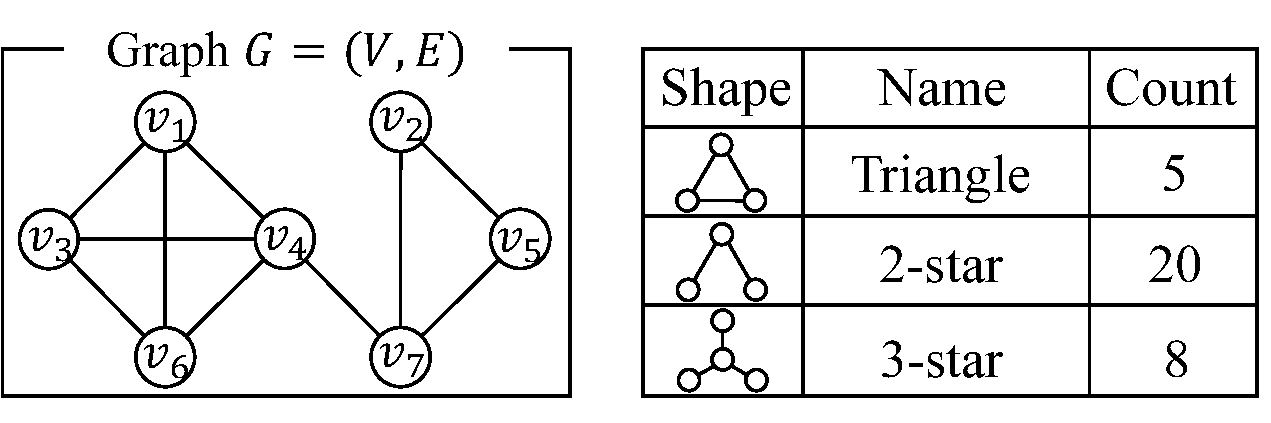
\includegraphics[width=0.9\linewidth]{fig/subgraph.pdf}

\caption[Example of subgraph counts.]{Example of subgraph counts.}
\label{chap1-fig:subgraph}
\end{figure}

In this paper, we consider LDP for graph data, and 
% propose solutions 
provide algorithms and theoretical performance guarantees
for calculating graph statistics in this model. 
In particular, we focus on counting triangles and $k$-stars -- the most basic and useful subgraphs. 
% such as triangles and $k$-stars. 
A triangle is a set of three nodes with three edges (we exclude automorphisms; i.e., \#closed triplets $= 3 \times$ \#triangles). 
A $k$-star consists of a central node connected to $k$ other nodes. 
Figure~\ref{chap1-fig:subgraph} shows an example of triangles and $k$-stars. 
Counting them is a fundamental task of analyzing the connection patterns in a graph, as 
% measures of centrality such as 
the clustering coefficient can be calculated from triangle and $2$-star counts as: $\frac{3 \times \text{\#triangles}}{\#2\text{-stars}}$ (in Figure~\ref{chap1-fig:subgraph}, $\frac{3 \times 5}{20} = 0.75$). 

When we look to protect privacy of relationship information modeled by edges in a graph, 
we need to pay attention to the fact 
% Note 
that some relationship information 
% about friendship (edges) 
could be leaked from subgraph counts. 
For example, 
% consider an adversary who 
suppose that user (node) $v_2$ in Figure~\ref{chap1-fig:subgraph} knows 
all edges connected to $v_2$ and 
all edges between $v_3, \ldots, v_7$ 
as background knowledge, and that $v_2$ wants to know who are friends with $v_1$. 
Then ``\#2-stars = 20'' reveals 
% to $v_2$ 
the fact that $v_1$ has three friends, and ``\#triangles = 5'' reveals 
% to $v_2$ 
the fact that the three friends of $v_1$ are $v_3$, $v_4$, and $v_6$. 
Moreover, a central server that holds all friendship information (i.e., all edges) may face data breaches, as explained above. 
Therefore, a private algorithm for counting subgraphs in the local model is highly beneficial to individual privacy.

%Counting subgraphs in the local model is very challenging. 
The main challenge in counting subgraphs in the local model is that existing techniques and their analysis do not directly apply. 
The existing work on LDP for tabular data assumes that 
each person's data 
is independently and identically drawn from an underlying distribution. 
% (see Section~\ref{chap1-sec:related}). 
In graphs, this is no longer the case; e.g., 
each triangle is not independent, 
because multiple triangles can involve the same edge; 
each $k$-star is not independent for the same reason. 
Moreover, complex inter-dependencies involving multiple people 
% is 
are 
possible in graphs. 
For example, each user cannot count triangles involving herself, because she cannot see edges between other users; 
e.g., 
% in Figure~\ref{chap1-fig:subgraph}, 
user 
% (node) 
$v_1$ cannot see an edge between $v_3$ and $v_4$ in Figure~\ref{chap1-fig:subgraph}. 

% This simultaneously presents both challenges and opportunities. 
We show that although these complex dependency among users introduces challenges, it also presents opportunities. Specifically, this kind of interdependency also implies that extra interaction between users and a data collector may be helpful depending on the prior responses. 
In this work, we investigate this issue and provide algorithms for accurately calculating subgraph counts under LDP. 
% counts that use various levels of interaction. 

\smallskip
\noindent{\textbf{Our contributions.}}~~In this paper, we provide 
% To our knowledge, we are the first to provide 
algorithms and corresponding performance guarantees for counting triangles and $k$-stars in graphs under edge Local Differential Privacy. Specifically, our contributions are as follows:
\begin{itemize}
    \item For triangles, we present two algorithms. The first is based on 
    Warner's RR (Randomized Response) \cite{Warner_JASA65} 
    and empirical estimation \cite{Kairouz_ICML16,Murakami_USENIX19,Wang_USENIX17}. 
    We then present a more sophisticated algorithm that uses an additional round of interaction between users and data collector. We provide upper-bounds on the estimation error for each algorithm, and show that the latter can  significantly reduce the estimation error. 
    
    \item For $k$-stars, we present a simple algorithm using the Laplacian mechanism. We analyze the upper-bound on the estimation error for this algorithm, and 
    show that it is order optimal in terms of the number of users among all LDP mechanisms that do not use additional interaction.
    
    \item We provide lower-bounds on the estimation error for 
    %estimating 
    general graph functions including triangle counts and $k$-star counts in the local model. These are stronger than known upper bounds in the centralized model, and illustrate the limitations of the local model over the central.
    
    \item Finally, we evaluate our algorithms on two real datasets, and show that 
    it is indeed possible to accurately estimate 
    subgraph counts in the local model. 
    %Our experimental results show that 
    %although the algorithms in the local model provide high estimation errors than those in the centralized model,  
    In particular, we show that 
    the interactive algorithm for triangle counts and the Laplacian algorithm for the $k$-stars provide small estimation errors when the number of users is large.
\end{itemize}

We implemented our algorithms with C/C++, and published them as open-source software \cite{LDPGraphStatistics}.

% \smallskip
% \noindent{\textbf{Related work.}}~~Here we explain the previous work related ours. 

%-------------------------------------------------------------------------------
\section{Related Work}
\label{sec:related}
%-------------------------------------------------------------------------------
% Here we review the prior work related to ours. 
% Here we review the previous work on graph DP (Differential Privacy), LDP (Local DP), and upper/lower-bounds.

\smallskip
\noindent{\textbf{Graph DP.}}~~DP on graphs has been widely studied, with most prior work being in the centralized model \cite{blocki2012johnson,Chen_PoPETs20,Day_SIGMOD16,Hay_ICDM09,Karwa_PVLDB11,Kasiviswanathan_TCC13,Nissim_STOC07,Raskhodnikova_arXiv15,Raskhodnikova_Encyclopedia16,Song_arXiv18,Wang_PAKDD13,Wang_TDP13}. 
% Some studies proposed algorithms for counting subgraphs in this model. 
% For example, Karwa \textit{et al.} \cite{Karwa_PVLDB11} proposed an algorithm for counting triangles and $k$-stars by adding the Cauchy noise to the true count. 
% Day \textit{et al.} \cite{Day_SIGMOD16} ...
% Kasiviswanathan \textit{et al.} \cite{Kasiviswanathan_TCC13} 
In this model, a number of algorithms have been proposed for releasing subgraph counts \cite{Karwa_PVLDB11,Kasiviswanathan_TCC13,Song_arXiv18}, degree distributions \cite{Day_SIGMOD16,Hay_ICDM09,Raskhodnikova_arXiv15}, eigenvalues and eigenvectors 
\cite{Wang_PAKDD13}, and synthetic graphs \cite{Chen_PoPETs20,Wang_TDP13}. 

% Algorithms for graph DP in the local model are much fewer, and \cite{Qin_CCS17,Ye_ICDE20,Zhang_USENIX20} are such examples. 
% Some studies proposed 
There has also been a handful of work on graph algorithms in the local DP model~\cite{Qin_CCS17,Sun_CCS19,Ye_ICDE20,Ye_TKDE21,Zhang_USENIX20}. 
For example, Qin \textit{et al.} \cite{Qin_CCS17} propose an algorithm for generating synthetic graphs. 
% while
% Ye \textit{et al.} \cite{Ye_ICDE20} 
% provide a method
% for graph metric estimation under LDP. 
% that perturbs 
% a neighbor list 
% an adjacency matrix by the RR (Randomized Response) 
% and each user's degree by the Laplacian noise. 
Zhang \textit{et al.} \cite{Zhang_USENIX20} propose an algorithm for software usage analysis under LDP, where a node represents a software component (e.g., function in a code) and an edge represents a control-flow between components. 
% None of these works focus on subgraph counts. 
Neither of these works focus on subgraph counts. 

Sun \textit{et al.} \cite{Sun_CCS19} propose an algorithm for counting subgraphs in the local model under the assumption that each user allows her friends to see all her connections. 
However, this assumption does not hold in many practical scenarios; e.g., a Facebook user can change her setting so that friends cannot see her connections. Therefore, we assume that each user knows only her friends rather than all of her friends' friends. 
The algorithms in \cite{Sun_CCS19} cannot be applied to this setting.

Ye \textit{et al.} \cite{Ye_ICDE20} propose a one-round algorithm for estimating graph metrics including the clustering coefficient. 
Here they apply Warner's RR (Randomized Response) to an adjacency matrix. 
However, it introduces a very large bias for triangle counts.
In \cite{Ye_TKDE21}, they propose a method for reducing the bias in the estimate of triangle counts. 
However, the method in \cite{Ye_TKDE21} introduces some approximation, and it is unclear whether their estimate is unbiased. 
In this paper, we propose a one-round algorithm for triangles that uses empirical estimation as a post-processing step, and prove that our estimate is unbiased. 
We also show in Appendix~\ref{sec:RR_emp} that our one-round algorithm significantly outperforms the one-round algorithm in \cite{Ye_ICDE20}. 
Moreover, we show in Section~\ref{sec:experiments} that our two-rounds algorithm significantly outperforms our one-round algorithm.

Our work also differs from \cite{Sun_CCS19,Ye_ICDE20,Ye_TKDE21} in that we provide lower-bounds on the estimation error.

% Our work differs from these in two ways: (i) our work provides algorithms and theoretical performance guarantees for subgraph counts, 
% (ii) we also 
% \colorB{provide} 
% lower-bounds on the estimation error. 
% We note that although Warner's RR (Randomized Response) has been applied to an adjacency matrix in \cite{Qin_CCS17,Ye_ICDE20} for different purposes than ours, it can be used for counting triangles. 
% However, it suffers from a very large estimation error. 
% Our one-round algorithm for triangles uses empirical estimation as a post-processing step, and we show in Appendix~\ref{sec:RR_emp} that this empirical estimation step significantly reduces the estimation error.

\smallskip
\noindent{\textbf{LDP.}}~~Apart from graphs, a number of works have looked at analyzing statistics (e.g., discrete distribution estimation\cite{Acharya_AISTATS19,Fanti_PoPETs16,Kairouz_ICML16,Kairouz_JMLR16,Murakami_USENIX19,Wang_USENIX17,Ye_ISIT17}, 
% and 
heavy hitters \cite{Bassily_STOC15,Bassily_NIPS17,Qin_CCS16}) under LDP. 
% Warner's RR \cite{Warner_JASA65}, $k$-ary RR \cite{Kairouz_ICML16}, RAPPOR \cite{Erlingsson_CCS14}, ...

However, they use LDP in the context of tabular data, and do not consider the kind of complex interdependency in graph data (as described in Section~\ref{sec:intro}). 
% it can happen that their algorithms do not work well for graph data which have complex interdependency. 
For example, the RR with empirical estimation is optimal in the low privacy regimes for estimating a distribution for tabular data \cite{Kairouz_ICML16,Kairouz_JMLR16}. 
We apply the RR and empirical estimation to counting triangles, and show that it is suboptimal and significantly outperformed by a more sophisticated 
two-rounds 
algorithm. 
% with more interaction between users and a data collector. 
% This example shows that directly applying existing LDP techniques does not work well. 

\smallskip
\noindent{\textbf{Upper/lower-bounds.}}~~Finally, we note that existing work on upper-bounds and lower-bounds cannot be directly applied to our setting. 
For example, there are upper-bounds
\cite{Acharya_AISTATS19,Kairouz_ICML16,Kairouz_JMLR16,Ye_ISIT17,Joseph_ArXiv19,Joseph_ArXiv19_Gauss} and
lower-bounds
\cite{Acharya_arXiv20,Duchi_ArXiv14,Duchi_ArXiv17,Joseph_ArXiv19,Duchi_ArXiv19,
Joseph_ArXiv19_Gauss, Joseph_SODA20} on the estimation error (or sample complexity) in 
% estimating a discrete distribution on personal data. 
distribution estimation of tabular data. 
% can be found in \cite{Acharya_AISTATS19,Duchi_ArXiv14,Kairouz_ICML16,Kairouz_JMLR16,Ye_ISIT17}. 
However, they assume that each original data value is independently sampled from an underlying distribution. 
They cannot be directly applied to our graph setting, because each triangle and each $k$-star involve multiple edges and are not independent (as described in Section~\ref{sec:intro}). 
% Acharya \textit{et al.} \cite{Acharya_arXiv20} provides lower-bounds on ...
Rashtchian \textit{et al.} \cite{Rashtchian_arXiv20} provide lower-bounds on communication complexity (i.e., number of queries) of vector-matrix-vector queries for estimating subgraph counts. 
However, their lower-bounds are not on the estimation error, and cannot be applied to our problem.

 %-------------------------------------------------------------------------------
\section{Preliminaries}
%-------------------------------------------------------------------------------
\label{chap1-sec:preliminaries}

% \subsection{Notations and Graphs}
% \label{chap1-sub:notations}
% \subsection{Graphs and Centralized Differential Privacy}
\subsection{Graphs and Differential Privacy}
\label{chap1-sub:graphs_CDP}
\noindent{\textbf{Graphs.}}~~Let $\nats$, $\nnints$, $\reals$, and $\nnreals$ be the sets of natural numbers, non-negative integers, real numbers, and non-negative real numbers, respectively. 
For $a \in \nats$, let $[a] = \{1, 2, \ldots, a\}$. 

We consider an undirected graph $G=(V,E)$, where 
$V$ is a set of nodes (i.e., users) and $E$ is a set of edges. 
Let $n \in \nats$ be the number of users in $V$, and let $v_i \in V$ the $i$-th user; i.e., $V=\{v_1,\ldots,v_n\}$. 
An edge $(v_i, v_j) \in E$ represents a relationship between users $v_i \in V$ and $v_j \in V$. 
% a node $v \in V$ represents a user and an edge $(u,v) \in E$ represents a relationship
% between users $u \in V$ and $v \in V$. 
The number of edges connected to a single node is called the \textit{degree} of the node. 
Let $d_{max} \in \nats$ be the \textit{maximum degree} (i.e., maximum number of edges connected to a node) in graph $G$. 
Let $\calG$ be the set of possible graphs 
% $G=(V,E)$ with $V=\{v_1,\ldots,v_n\}$. 
$G$ on $n$ users. 
A graph $G \in \calG$ can be represented as a symmetric adjacency matrix $\bmA=(a_{i,j}) \in \{0,1\}^{n \times n}$, where $a_{i,j}=1$ if $(v_i,v_j) \in E$ and $a_{i,j}=0$ otherwise.

% \subsection{Centralized Differential Privacy}
% \label{chap1-sub:CDP}
\smallskip
% \noindent{\textbf{Centralized DP.}}~~
\noindent{\textbf{Types of DP.}}~~
DP (Differential Privacy) \cite{DP,Dwork_ICALP06} is known as a gold standard for data privacy. 
According to the underlying architecture, DP can be divided into two 
% categories: 
types: 
\textit{centralized DP} and \textit{LDP (Local DP)}. 
% the one in the centralized (or global) model and the one in the local model. 
% In the centralized model, a trusted database 
Centralized DP assumes the centralized model, where a ``trusted'' data collector 
% database administrator 
collects the original personal data from all users and obfuscates a query (e.g., counting query, histogram query) on the set of personal data. 
% In contrast, 
LDP assumes the local model, where each user does not trust even the data collector. 
In this model, each user obfuscates a query on her personal data by herself and sends the obfuscated data to the data collector. 
% We begin by explaining centralized DP on graphs.

% There are two types of DP on graphs: 
If the data are represented as a graph, we can consider two types of DP: 
% centralized DP: 
% If the input is a graph, we can consider two types of DP: 
% centralized DP: 
% \textit{edge centralized DP} and \textit{node centralized DP} \cite{Hay_ICDM09}. 
\textit{edge DP} and \textit{node DP} \cite{Hay_ICDM09,Raskhodnikova_Encyclopedia16}. 
% We refer to edge DP and node DP in the centralized model as edge centralized DP and node centralized DP, respectively. 
Edge DP considers two neighboring graphs $G, G' \in \calG$ that differ in one edge. 
In contrast, node DP considers two neighboring graphs $G, G' \in \calG$ in which $G'$ is obtained from $G$ by adding or removing one node along with its adjacent edges. 
% Although node DP guarantees stronger privacy than edge DP, 
% it is much harder to attain. 

% Zhang \textit{et al.} \cite{Zhang_USENIX20} proposed an algorithm for software usage analysis with node DP in the local model, where a node represents a software component 
% and an edge represents a control-flow between components. 
% However, we consider a totally different problem, where each node represents a user (rather than a software component). 
Although Zhang \textit{et al.} \cite{Zhang_USENIX20} consider node DP in the local model where each node represents a software component, we consider a totally different problem where each node represents a user. 
% (rather than a software component). 
In the latter case, 
% achieving node DP in the local model is extremely difficult 
% because each user needs to hide the \textit{existence of herself} along with her all edges against the data collector. 
node DP requires us to hide the \textit{existence of each user} along with her all edges. 
% against the data collector. 
However, many applications in the local model send the identity of each user to a server. 
For example, 
we can consider a mobile application 
% that asks a users how many friends she met today and sends noisy counts and her user ID to a server. 
that sends to a server how many friends a user met today along with her user ID. 
In this case, the user may not mind sending her user ID, 
% (i.e., who the user is), 
but may want to hide her edge information (i.e., who she met today). 
Although we cannot use node DP in such applications, we can use edge DP to deny the presence/absence of each edge (friend). 
Thus we focus on edge DP in the same way as \cite{qin2017generating,Sun_CCS19,Ye_ICDE20,Ye_TKDE21}. 

% We refer to edge DP in the centralized model as \textit{edge centralized DP}, and explain it in detail below.
Below we explain edge DP in the centralized model. 

\smallskip
\noindent{\textbf{Centralized DP.}}~~We call edge DP in the centralized model \textit{edge centralized DP}. 
% Edge centralized DP is 
% Edge centralized DP considers two neighboring graphs that differ in one edge. 
Formally, it is defined as follows:

\begin{definition} [$\epsilon$-edge centralized DP] \label{chap1-def:edge_CDP} 
Let $\epsilon \in \nnreals$. 
A randomized algorithm $\calM$ with domain $\calG$ provides \emph{$\epsilon$-edge centralized DP} 
if for any two 
neighboring 
graphs $G, G' \in \calG$ that differ in one edge and any $S \subseteq \mathrm{Range}(\calM)$, 
\begin{align}
\Pr[\calM(G) \in S] \leq e^\epsilon \Pr[\calM(G') \in S].
\label{chap1-eq:edge_CDP}
\end{align}
\end{definition}
Edge centralized DP guarantees that an adversary who has observed the output of $\calM$ cannot determine whether it is come from $G$ or $G'$ with a certain degree of confidence. 
The parameter $\epsilon$ is called the \textit{privacy budget}. 
% and controls the amount of information leaked from the output of $\calM$. 
If $\epsilon$ is close to zero, then $G$ and $G'$ are almost equally likely, which means that an edge in $G$ is strongly protected. 

We also note that edge DP can be 
% easily extended 
used 
to protect $k\in\nats$ edges by using 
the notion of group privacy \cite{DP}.
Specifically, if $\calM$ provides $\epsilon$-edge centralized DP, then for any two graphs $G, G' \in \calG$ that differ in $k$ edges and any $S \subseteq \mathrm{Range}(\calM)$, we obtain: 
$\Pr[\calM(G) \in S] \leq e^{k\epsilon} \Pr[\calM(G') \in S]$; i.e., $k$ edges are protected with privacy budget $k\epsilon$.

\subsection{Local Differential Privacy}
\label{chap1-sub:LDP}
LDP (Local Differential Privacy) \cite{Kasiviswanathan_FOCS08,Duchi_FOCS13} is a privacy metric to protect personal data of each user in the local model. 
LDP has been originally introduced to protect each user's data record that is independent from the other records. 
However, in a graph, each edge is connected to two users. 
Thus, when we define edge DP in the local model, 
% i.e., \textit{edge LDP}, 
we should consider what we want to protect. 
In this paper, we consider two definitions of edge DP in the local model: \textit{edge LDP} in \cite{qin2017generating} and 
% \textit{entire edge LDP} 
\textit{relationship DP} 
introduced in this paper. 
Below, we will explain these two definitions in detail. 

% Applying LDP to a graph is not straightforward 
% because adding or removing one edge will affect neighbor lists of two users. 

\smallskip
\noindent{\textbf{Edge LDP.}}~~Qin \textit{et al.} \cite{qin2017generating} defined edge LDP based on a user's \textit{neighbor list}. 
% use the definition of edge LDP in \cite{qin2017generating}, which is based on a user's \textit{neighbor list}. 
Specifically, 
% given a user in $V$, 
% let $b_i \in \{0,1\}$ be a binary bit that takes $1$ if there is an edge between the user and user $v_i \in V$ and $0$ otherwise. 
% Let 
% $\bmb = (b_1, \ldots, b_n) \in \{0,1\}^n$ be a neighbor list. 
% Let $\bma_i = (a_{i,1}, \ldots, a_{i,n}) \in \{0,1\}^n$ be the $i$-th row of the adjacency matrix $\bmA$. 
% Note that a graph $G$ can be represented as neighbor lists $\textbf{a}_1, \ldots, \textbf{a}_n$, and $\bma_i$ is a neighbor list of user $v_i$. 
let $\bma_i = (a_{i,1}, \ldots, a_{i,n}) \in \{0,1\}^n$ be a neighbor list of user $v_i$. 
Note that $\bma_i$ is the $i$-th row of the adjacency matrix $\bmA$ of graph $G$. 
In other words, graph $G$ can be represented as neighbor lists $\textbf{a}_1, \ldots, \textbf{a}_n$. 

Then edge LDP is defined as follows: 

\begin{definition} [$\epsilon$-edge LDP \cite{qin2017generating}] \label{chap1-def:edge_LDP} 
Let $\epsilon \in \nnreals$. 
For any $i \in [n]$, let $\calR_i$ with domain $\{0,1\}^n$ be a randomized algorithm of user $v_i$. 
% A randomized algorithm $\calR$ with domain $\{0,1\}^n$ 
$\calR_i$ 
provides \emph{$\epsilon$-edge LDP} 
if for any two neighbor lists 
% $\bmb, \bmb' \in \{0,1\}^n$ 
$\bma_i, \bma'_i \in \{0,1\}^n$ 
that differ in one bit and any 
% $S \subseteq \mathrm{Range}(\calR)$, 
$S \subseteq \mathrm{Range}(\calR_i)$, 
\begin{align}
% \Pr[\calR(\bmb) \in S] \leq e^\epsilon \Pr[\calR(\bmb') \in S].
\Pr[\calR_i(\bma_i) \in S] \leq e^\epsilon \Pr[\calR_i(\bma'_i) \in S].
\label{chap1-eq:edge_LDP}
\end{align}
\end{definition}
Edge LDP in Definition~\ref{chap1-def:edge_LDP} protects 
a single bit in a neighbor list with privacy budget $\epsilon$. 
% For example, consider an application that asks a users how many friends she met today and sends noisy counts and her user ID to a server. 
% In this case, the user would not mind sending her identity 
% % (i.e., who the user is), 
% but want to hide who she met today (i.e., who are her neighbors). 
% Edge LDP can be used to deny the presence/absence of one neighbor.
As with edge centralized DP, edge LDP can also be 
% extended 
used 
to protect $k \in \nats$ 
bits in a neighbor list 
% neighbors 
by using group privacy; i.e., $k$ bits in a neighbor list are protected with privacy budget $k\epsilon$. 

% We can consider an application of the randomized algorithm $\calR$ with input $\bmb$ as follows. 
% For example, suppose that a data collector asks each user to send some query (e.g., number of friends, who are friends) on her neighbor list $\bmb$. 
% To protect $\bmb$, each user obfuscates her answer to the query by using $\calR$ and sends the noisy answer to the data collector. 
% Then the data collector estimates some graph statistics 
% (e.g., number of triangles, clustering coefficient) 
% based on the noisy answer from each user. 

\smallskip
% \noindent{\textbf{RNL (Randomized Neighbor List).}}~~
\noindent{\textbf{RR (Randomized Response).}}~~As a simple example of a randomized algorithm 
% $\calR$ 
$\calR_i$ 
providing $\epsilon$-edge LDP, we explain 
% the 
Warner's RR (Randomized Response) \cite{Warner_JASA65} applied to a neighbor list, 
which is called 
% the RNL (Randomized neighbor List) 
the randomized neighbor list in \cite{qin2017generating}. 
% and is also used in \cite{Ye_ICDE20}. 

Given a neighbor list 
% $\bmb \in \{0,1\}^n$, 
$\bma_i \in \{0,1\}^n$, 
% the RNL 
this algorithm 
outputs a noisy neighbor lists 
% $\bms = (s_1, \ldots, s_n) \in \{0,1\}^n$ 
$\bmb = (b_1, \ldots, b_n) \in \{0,1\}^n$ 
by flipping each bit in 
% $\bmb$ 
$\bma_i$ 
with probability $p = \frac{1}{e^\epsilon + 1}$; i.e., for each $j \in [n]$, 
% $s_i \neq b_i$ with probability $p$ and $s_i = b_i$ with probability $1-p$. 
$b_j \neq a_{i,j}$ with probability $p$ and $b_j = a_{i,j}$ with probability $1-p$. 
Since 
% $\Pr[\calR(\bmb) \in S]$ and $\Pr[\calR(\bmb') \in S]$ 
$\Pr[\calR(\bma_i) \in S]$ and $\Pr[\calR(\bma'_i) \in S]$ 
in (\ref{chap1-eq:edge_LDP}) differ by $e^\epsilon$ for 
% $\bmb$ and $\bmb'$ 
$\bma_i$ and $\bma'_i$ 
that differ in one bit, 
% It is easy to verify that 
% the RNL 
this algorithm 
provides $\epsilon$-edge LDP. 

\smallskip
% \noindent{\textbf{Remark.}}~~
% \noindent{\textbf{Alternative definition of edge LDP.}}~~
\noindent{\textbf{Relationship DP.}}~~In graphs such as social networks, 
% For graph datasets, 
it is usually the case that two users share knowledge of the presence of an edge between them. 
% For example, in social networks it is usually the norm that
% friendship status is known by both parties.
% With the goal of hiding their mutual edge, 
To hide their mutual edge, 
we must consider
that both user's outputs can leak information. 
We introduce a DP definition called relationship DP that hides \textit{one entire edge in graph $G$ during the whole process:}
% avoid confusion. 
% For example, divide a graph $G$ into disjoint sets $(G_1, \ldots, G_n)$ such that user $v_i$ can see $G_i$. 
% For example, 

% Then 
% We define relationship DP as follows: 
% (we call this version of edge LDP \textit{entire edge LDP} to avoid confusion):

\begin{definition} [$\epsilon$-relationship DP] 
% [$\epsilon$-entire edge LDP] 
\label{chap1-def:entire_edge_LDP} 
Let $\epsilon \in \nnreals$. 
% Let $\calR_1, \ldots, \calR_n$ be randomized algorithms, each of which is with domain $\{0,1\}^n$. 
A tuple of randomized algorithms $(\calR_1, \ldots, \calR_n)$, 
each of which is with domain $\{0,1\}^n$, 
provides 
% \emph{$\epsilon$-entire edge LDP} 
\emph{$\epsilon$-relationship DP} 
if for any two 
neighboring 
graphs $G, G' \in \calG$ that differ in one edge and any $S \subseteq \mathrm{Range}(\calR_1) \times \ldots \times \mathrm{Range}(\calR_n)$, 
\begin{align}
&\Pr[(\calR_1(\bma_1), \ldots, \calR_n(\bma_n)) \in S] \nonumber\\
&\leq e^\epsilon \Pr[(\calR_1(\bma'_1), \ldots, \calR_n(\bma'_n)) \in S],
\label{chap1-eq:entire_edge_LDP}
\end{align}
where $\bma_i$ (resp.~$\bma'_i$) $\in \{0,1\}^n$ is the $i$-th row of the adjacency matrix of graph $G$ (resp.~$G'$).
\end{definition}

Relationship DP is the same as \textit{decentralized DP} in \cite{Sun_CCS19} except that the former (resp.~latter) assumes that each user knows only her friends (resp.~all of her friends' friends).

% Relationship DP is distinct from edge LDP because 
Edge LDP assumes that 
% user $v_i$ being connected to user $v_j$ 
user $v_i$'s edge connected to user $v_j$ 
and 
% user $v_j$ being connected to user $v_i$ 
user $v_j$'s edge connected to user $v_i$ 
are different secrets, with user $v_i$ knowing the former and user $v_j$ knowing the latter. 
% As we stated above, the presence of an edge is usually known by both its users. 
Relationship DP assumes that the two secrets are the same.

% Since secrets are shared among two users, 
Note that 
the threat model of relationship DP is 
% not quite 
different from 
that of 
% local DP: 
LDP -- 
some amount of trust must be given to the other users 
in relationship DP. 
Specifically, user $v_i$ must trust user $v_j$ to not leak information
about their shared edge. If $k \in \nats$ users decide not to follow their protocols, 
then up to $k$ edges incident to user $v_i$ may be compromised. This trust model
is stronger than 
% local DP, 
LDP, 
which assumes nothing about what other users 
% may 
do,
but is much weaker than centralized DP in which 
% all information of a user is 
all edges are 
in the hands of the central party.

Other than the differing threat models, relationship DP and edge LDP are quite closely related:

\begin{proposition} \label{chap1-prop:edge_LDP_entire_edge_LDP} 
If randomized algorithms $\calR_1, \ldots, \calR_n$ provide $\epsilon$-edge LDP, 
then $(\calR_1, \ldots, \calR_n)$ provides $2\epsilon$-relationship DP.
\end{proposition}

\begin{proof}
The existence of edge $(v_i, v_j) \in E$ affects two elements $a_{i,j}, a_{j,i} \in \{0,1\}$ in the adjacency matrix $\bmA$. 
  Then by group privacy~\cite{DP}, Proposition~\ref{chap1-prop:edge_LDP_entire_edge_LDP} holds.
\end{proof}

% The existence of edge $(v_i, v_j) \in E$ affects two elements $a_{i,j}, a_{j,i} \in \{0,1\}$ in the adjacency matrix $\bmA$. 
% Therefore, by the composition theorem \cite{DP}, if all of the randomized algorithms $\calR_1, \ldots, \calR_n$ provide $\epsilon$-edge LDP in Definition~\ref{chap1-def:edge_LDP}, 
% then the tuple $(\calR_1, \ldots, \calR_n)$ provides $2\epsilon$-entire edge LDP in Definition~\ref{chap1-def:entire_edge_LDP}; i.e., the privacy budget is at most doubled. 

Proposition~\ref{chap1-prop:edge_LDP_entire_edge_LDP} states that when we want to protect one edge as a whole, the privacy budget is at most doubled. 
Note, however, that 
% the privacy budget is not changed for some randomized algorithms. 
some randomized algorithms do not have this doubling issue. 
For example, we can apply the RR to the $i$-th neighbor list $\bma_i$ so that $\calR_i$ outputs noisy bits 
% $(t_{i+1}, \ldots, t_n) \in \{0,1\}^{n-i}$ 
% $(t_1, \ldots, t_{i-1}) \in \{0,1\}^{i-1}$ 
$(b_1, \ldots, b_{i-1}) \in \{0,1\}^{i-1}$ 
for only users 
% $v_{i+1}, \ldots, v_n$ with larger user IDs; 
$v_1, \ldots, v_{i-1}$ with smaller user IDs; 
i.e., 
% In other words, we can modify the RNL as follows: 
for each 
% $j \in \{i+1, \ldots, n\}$, 
$j \in \{1, \ldots, i-1\}$, 
% $\calR_i$ outputs $(t_{i+1}, \ldots, t_n) \in \{0,1\}^{n-i}$, where 
% $t_j \neq a_{i,j}$ with probability $p = \frac{1}{e^\epsilon + 1}$ and $t_j = a_{i,j}$ with probability $1-p$. 
$b_j \neq a_{i,j}$ with probability $p = \frac{1}{e^\epsilon + 1}$ and $b_j = a_{i,j}$ with probability $1-p$. 
In other words, we can extend 
% the RNL 
the RR for a neighbor list 
so that $(\calR_1, \ldots, \calR_n)$ outputs only 
% the upper triangular part 
the lower triangular part 
of the noisy adjacency matrix. 
Then all of $\calR_1, \ldots, \calR_n$ provide $\epsilon$-edge LDP. 
In addition, the existence of edge $(v_i, v_j) \in E$ 
% $(i < j)$ 
$(i > j)$ 
affects only one element $a_{i,j}$ in 
% the upper triangular part 
the lower triangular part 
of $\bmA$. 
Thus, $(\calR_1, \ldots, \calR_n)$ provides $\epsilon$-relationship DP (not $2\epsilon$). 
% Note that this extended algorithm requires each user to know who are users with larger user IDs. 
% One way to do so is to send user IDs of $n$ users from the data collector to each user in advance. 

Our proposed algorithm in Section~\ref{chap1-sub:two_rounds} also has this property; i.e., 
it provides both $\epsilon$-edge LDP and $\epsilon$-relationship DP. 
% can also be extended so that the tuple $(\calR_1, \ldots, \calR_n)$ provides $\epsilon$-entire edge LDP (not $2\epsilon$), given that each user knows users with larger user IDs. 
% We describe the extended algorithm in Appendix~\ref{chap1-sec:modified_two_rounds}. 


% \smallskip
% \noindent{\textbf{Global/local sensitivity.}}~~
% \subsection{Global Sensitivity and Local Sensitivity}
\subsection{Global Sensitivity}
\label{chap1-sub:sensitivity}
In this paper, we use the notion of global sensitivity \cite{DP} to provide edge centralized DP or edge LDP.
% In this paper, we use the local sensitivity \cite{Nissim_STOC07} to provide 
% edge centralized DP or edge LDP with small noise.
% Here we explain the global sensitivity \cite{DP} and the local sensitivity \cite{Nissim_STOC07}. 

Let $\calD$ be the set of possible input data of a randomized algorithm. 
In edge centralized DP, $\calD = \calG$. 
In edge LDP, $\calD = \{0,1\}^n$. 
Let $f: \calD \rightarrow \reals$ be a function that takes data $D \in \calD$ as input and outputs some statistics $f(D) \in \reals$ about the data. 
% $f: \calG \rightarrow \reals$ 
% be a function that takes a graph $G \in \calG$ as input and outputs some graph statistics $f(G) \in \reals$. 
% Assume that we want to estimate some graph statistics $f(G) \in \reals$. 
The most basic method for providing DP is to add the Laplacian noise proportional to the global sensitivity \cite{DP}.

\begin{definition} [Global sensitivity] \label{chap1-def:global_sen} 
The global sensitivity of a function $f: \calD \rightarrow \reals$ is given by:
\begin{align*}
GS_f = \underset{D,D' \in \calD: D \sim D'}{\max} |f(D) - f(D')|,
%\label{chap1-eq:global_sen}
\end{align*}
where $D \sim D'$ represents that $D$ and $D'$ are neighbors; i.e., they differ in one edge in edge centralized DP, and differ in one bit in edge LDP.
\end{definition}

% For example, consider a function that 
% takes a neighbor list $\bma_i$ of user $v_i$ and outputs the number of $2$-stars of which she is a center. 
% Since adding 

% For $b \in \nnreals$, let $\Lap(b)$ be a random variable that represents the Laplacian noise with mean $0$ and scale $b$. 
% Then for $\epsilon \in \nnreals$, $f(D) + \Lap(GS_f/\epsilon)$ provides $\epsilon$-DP. 
% Here $\epsilon$-DP can be instantiated by $\epsilon$-edge centralized DP or $\epsilon$-edge LDP. 

% In graph privacy, the global sensitivity $GS_f$ can be very large. 
% since adding one edge in $G$ can result in 
% the increase of $n-2$ triangles, 
% $GS_f = 2 \binom{n}{k-1}$ for $k$-star counts and 
% $GS_f = n-2$ for triangle counts under edge centralized DP. 
% Similarly, the global sensitivity is large for $k$-star counts.
% In practice, the global sensitivity $GS_f$ can be very large. 
In graphs, the global sensitivity $GS_f$ can be very large. 
For example, adding one edge may result in the increase of triangle (resp.~$k$-star) counts by $n-2$ (resp.~$\binom{n}{k-1}$). 

One way to significantly reduce the global sensitivity is to use \textit{graph projection} \cite{Day_SIGMOD16,Kasiviswanathan_TCC13,Raskhodnikova_arXiv15}, which removes some neighbors from a neighbor list so that the maximum degree $d_{max}$ is upper-bounded by a predetermined value $\td_{max} \in \nnints$. 
By using the graph projection with $\td_{max} \ll n$, we can enforce small global sensitivity; e.g., the global sensitivity of triangle (resp.~$k$-star) counts is at most $\td_{max}$ (resp.~$\binom{\td_{max}}{k-1}$) after the projection. 
% This technique is also known as \textit{clipping} \cite{Abadi_CCS16,Thakkar_arXiv19}.
% so that the local sensitivity is upper-bounded by the private estimate of $LS_f(D)$. 

Ideally, we would like to set $\td_{max} = d_{max}$ to avoid removing neighbors from a neighbor list (i.e., to avoid the loss of utility). 
However, the maximum degree $d_{max}$ can leak some information about the original graph $G$. 
In this paper, we address this issue by privately estimating $d_{max}$ with edge LDP and then using the private estimate of $d_{max}$ as $\td_{max}$.
% We call 
This technique 
is also known as 
\textit{adaptive clipping} 
% , and is studied for determining an appropriate threshold of the gradient $l_2$-norm 
% This is also studied for 
in differentially private stochastic gradient descent (SGD) \cite{Pichapati_arXiv19,Thakkar_arXiv19}.


% Nissim \textit{et al.} \cite{Nissim_STOC07} introduced a local measure of sensitivity called the \textit{local sensitivity} to address this issue. 

% \begin{definition} [Local sensitivity \cite{Nissim_STOC07}] \label{chap1-def:local_sen} 
% The local sensitivity of a function $f: \calD \rightarrow \reals$ at $D \in \calD$ is given by:
% \begin{align*}
% LS_f(D) = \underset{D' \in \calD: D \sim D'}{\max} |f(D) - f(D')|.
% \end{align*}
% \end{definition}
% Note that $GS_f = \max_{D \in \calD} LS_f(D)$. 
% In practice, $LS_f(D)$ can be much smaller than $GS_f$. 
% For example, the local sensitivity of triangle counts in $G$ is at most the maximum degree $d_{max}$, which is much smaller than $GS_f = n-2$ when $G$ is sparse. 

% The local sensitivity $LS_f(D)$ cannot be directly used, 
% because the noise magnitude can leak some information about $G$. 
% Karwa \textit{et al.} \cite{Karwa_PVLDB11} showed that in the centralized graph model, adding the Cauchy noise (rather than the Laplacian noise) with the local sensitivity 
% to $k$-star or triangle counts in $G$ provides $\epsilon$-edge centralized DP under some conditions. 
% However, in the local graph model, it is even difficult for users to know the local sensitivity itself. 
% In this paper, we address this issue by privately estimating 
% $LS_f(D)$ 
% with edge LDP and then applying \textit{graph projection} \cite{Day_SIGMOD16,Kasiviswanathan_TCC13,Raskhodnikova_arXiv15}, which removes some neighbors from a neighbor list, 
% so that the local sensitivity is upper-bounded by the private estimate of $LS_f(D)$. 

% if we provide $\epsilon_0$-DP for $LS_f(D)$ by adding noise, adding the noisy $\Lap(LS_f/\epsilon)$ to $f(D)$ provides $(\epsilon_0 + \epsilon)$-DP by the composition theorem \cite{DP}.



\subsection{Graph Statistics and Utility Metrics}
\label{chap1-sub:graph_statistics}

\noindent{\textbf{Graph statistics.}}~~We consider a graph function that takes a graph $G \in \calG$ as input and outputs some graph statistics. 
% Here we consider two types of graph statistics. 
% The first type is \textit{subgraph counts}. 
Specifically, 
let $f_\triangle: \calG \rightarrow \nnints$ be a graph function that outputs the number of triangles in $G$. 
For $k \in \nats$, let $f_{k\star}: \calG \rightarrow \nnints$ be a graph function that outputs the number of $k$-stars in $G$. 
% We call $f_\triangle$ and $f_{k\star}$ the \textit{triangle function} and \textit{$k$-star function}, respectively. 
For example, if a graph $G$ is as shown in Figure~\ref{chap1-fig:subgraph}, then $f_\triangle(G) = 5$, $f_{2\star}(G) = 20$, and $f_{3\star}(G) = 8$. The clustering coefficient can also be calculated from $f_\triangle(G)$ and $f_{2\star}(G)$ as: $\frac{3 f_\triangle(G)}{f_{2\star}(G)} = 0.75$. 

% The second type of graph statistics is \textit{degree information}. 
% For this type of statistics, we define the following basic function. 
% For $i \in [n]$, let $f_{d_i}: \calG \rightarrow \nnints$ be a graph function that 
% outputs a degree (i.e., the number of edges) of user $v_i$ in $G$. 
% We call $f_{d_i}$ the \textit{degree function}. 
% In Figure~\ref{chap1-fig:subgraph}, 
% $f_{d_1}(G) = 3, f_{d_2}(G) = 2, \ldots, f_{d_7}(G) = 3$. 
% A degree distribution can be easily calculated from 
% $f_{d_1}(G), \ldots, f_{d_n}(G)$. 
% In Figure~\ref{chap1-fig:subgraph}, the degree distribution can be expressed as $(0, 0, \frac{2}{7}, \frac{4}{7}, \frac{1}{7})$, where the $i$-th value represents the ratio of $(i-1)$ in 
% $f_{d_1}(G), \ldots, f_{d_n}(G)$; 
% e.g., the 5th value is $\frac{1}{7}$ because ``4'' appears once ($f_{d_4}(G) = 4$). 

% \begin{table}[t]
% \caption{Basic notations in this paper.} 
% \centering
% \hbox to\hsize{\hfil
% \begin{tabular}{l|l}
% \hline
% Symbol		&	Description\\
% \hline
% $G=(V,E)$   &	    Graph with $n$ nodes (users) $V$ and edges $E$\\
% $v_i$       &       $i$-th user in $V$.\\
% $d_{max}$   &       Maximum degree of $G$.\\
% $\calG$     &       Set of possible graphs on $n$ users.\\
% $\bmA$	    &		Adjacency matrix.\\
% $\bma_i$	&		$i$-th row of $\bmA$ (i.e., neighbor list of $v_i$).\\
% $\calR_i$     &       Randomized algorithm on $\bma_i$.\\
% $f_\triangle(G)$   &  Number of triangles in $G$.\\
% $f_{k\star}(G)$    &  Number of $k$-stars in $G$.\\
% \hline
% \end{tabular}
% \hfil}
% \label{chap1-tab:notations}
% \end{table}

\begin{table}[t]
\caption[Basic notations in this paper.]{Basic notations in this paper.} 
\centering
\hbox to\hsize{\hfil
\begin{tabular}{l|l}
\hline
Symbol		&	Description\\
\hline
$n$         &	    Number of users.\\
$G=(V,E)$   &	    Graph with $n$ nodes (users) $V$ and edges $E$.\\
$v_i$       &       $i$-th user in $V$.\\
$d_{max}$   &       Maximum degree of $G$.\\
$\td_{max}$   &       Upper-bound on $d_{max}$ (used for projection).\\
$\calG$     &       Set of possible graphs on $n$ users.\\
$\bmA=(a_{i,j})$	    &		Adjacency matrix.\\
$\bma_i$	&		$i$-th row of $\bmA$ (i.e., neighbor list of $v_i$).\\
$\calR_i$     &       Randomized algorithm on $\bma_i$.\\
$f_\triangle(G)$   &  Number of triangles in $G$.\\
$f_{k\star}(G)$    &  Number of $k$-stars in $G$.\\
\hline
\end{tabular}
\hfil}
\label{chap1-tab:notations}
\end{table}

% \colorB{We show the basic notations in Table~\ref{chap1-tab:notations} of Appendix~\ref{chap1-sec:notations}.} 
Table~\ref{chap1-tab:notations} shows the basic notations used in this paper.

\smallskip
\noindent{\textbf{Utility metrics.}}~~We use the $l_2$ loss (i.e., squared error) \cite{Kairouz_ICML16,Wang_USENIX17,Murakami_USENIX19} and the relative error \cite{Bindschaedler_SP16,Chen_CCS12,Xiao_SIGMOD11} as utility metrics. 

% In our theoretical analysis, we use the $l_2$ loss between the true value and the estimate. 
Specifically, let 
% $\hf: \calG \rightarrow \reals$ be a function that takes a graph $G \in \calG$ as input and outputs an estimate $\hf(G) \in \reals$ of graph statistics $f(G) \in \nnints$.
$\hf(G) \in \reals$ be an estimate of graph statistics $f(G) \in \reals$. 
Here $f$ can be instantiated by 
% $f_\triangle$, $f_{k\star}$, or $f_{d_i}$; 
$f_\triangle$ or $f_{k\star}$; 
i.e., 
% $\hf_\triangle(G)$, $\hf_{k\star}(G)$, and $\hf_{d_i}(G)$ are the estimates of $f_\triangle(G)$, $f_{k\star}(G)$, and $f_{d_i}(G)$, respectively. 
$\hf_\triangle(G)$ and $\hf_{k\star}(G)$ are the estimates of $f_\triangle(G)$ and $f_{k\star}(G)$, respectively. 
Let $l_2^2$ be the $l_2$ loss function, which maps the estimate $\hf(G)$ and the true value $f(G)$ to the $l_2$ loss; i.e., $l_2^2(\hf(G), f(G)) = (\hf(G) - f(G))^2$. 
% \begin{align*}
% l_2^2(\hf(G), f(G)) = (\hf(G) - f(G))^2. 
% \end{align*}
% We denote the estimates of $f_\triangle(G)$, $f_{k\star}(G)$, and $f_{d_i}(G)$ by $\hf_\triangle(G)$, $\hf_{k\star}(G)$, and $\hf_{d_i}(G)$, respectively. 
% When we estimate graph statistics based on the output of 
% 
Note that when we use a randomized algorithm providing edge LDP (or edge centralized DP), $\hf(G)$ depends on the randomness in the algorithm. 
In our theoretical analysis, we analyze the expectation of the $l_2$ loss over 
the randomness, as with \cite{Kairouz_ICML16,Wang_USENIX17,Murakami_USENIX19}. 
% possible realization of $\hf(G)$.
% For 
% and analyze their $l_2$ loss in our theoretical analysis in the same way as . 
% In our experiments, we replace the expectation of the $l_2$ loss with the sample mean of the $l_2$ loss over multiple realizations of 

When $f(G)$ is large, the $l_2$ loss can also be large. 
Thus in our experiments, we also evaluate the relative error, along with the $l_2$ loss. 
The relative error is defined as: $\frac{|\hf(G) - f(G)|}{\max\{f(G), \eta\}}$, where $\eta \in \nnreals$ is a very small positive value. 
Following the convention \cite{Bindschaedler_SP16,Chen_CCS12,Xiao_SIGMOD11}, we set $\eta = 0.001n$ 
for $f_\triangle$ and $f_{k\star}$. 
% Ideally, the relative error should be small than $1$.

%-------------------------------------------------------------------------------
\section{Algorithms}
\label{chap1-sec:algorithms}
%-------------------------------------------------------------------------------
% When the data collector does not have access to the adjacency matrix
% $\bmA$, a unique communication challenge arises. 
In the local model, 
% There 
there 
are several ways 
% in which we may 
to 
model how the data collector interacts with 
the users~\cite{Duchi_FOCS13,Joseph_SODA20,Qin_CCS17}.
The simplest model 
would be 
% is 
to assume that 
% \colorB{each user $v_i$ independently runs the randomized algorithm $\calR_i$ on the neighbor list $\bma_i$ and sends the output $\calR_i(\bma_i)$ to the data collector.} 
the data collector sends 
% one 
a 
query $\calR_i$ to each user $v_i$ once, 
and then 
% and no communication among users occurs.
% The data collector would then receive 
% receives an answer $\calR_i(\bma_i)$ from each user $v_i$. 
each user $v_i$ independently sends an answer $\calR_i(\bma_i)$ to the data collector. 
% independent copies of the random variables
% $(\calR_1(\bma_1), \ldots, \calR_n(\bma_n))$. 
In this model, there is one-round interaction between each user and the data collector. 
We call this the
% \textit{non-interactive graph LDP model}. 
\textit{one-round LDP model}. 
% This model is also called the \textit{non-interactive model}~\cite{Duchi_FOCS13,Joseph_SODA20} because there is no interaction among users (note that there is interaction between each user and the data collector). 
For example, the RR 
%(Randomized Response) 
for a neighbor list in Section~\ref{chap1-sub:LDP} assumes this model.

However, in certain cases it may be possible 
for the data collector to send a query to each user multiple times. 
This could allow for more powerful queries that result in more accurate 
% analysis of graph statistics 
subgraph counts 
\cite{Sun_CCS19} 
or more accurate synthetic graphs~\cite{Qin_CCS17}. 
We call this the \textit{multiple-rounds LDP model}. 
% For example, a synthetic graph generation technique in the two-rounds LDP model has been proposed in~\cite{Qin_CCS17}.

% Note that we assume interaction between each user and the data collector, and do not assume interaction among users in both the one-round and multiple-rounds LDP models.}

% to ask user $i$ an interactive
% query $\calR_i$; namely, it may
% depend on $(\calR_1(\bma_1), \ldots, \calR_{i-1}(\bma_{i-1}))$.
% This could allow for more powerful queries, but the drawback compared to the
% non-interactive graph LDP model
% is that the data collector must wait for user $i-1$ to 
% respond before querying user $i$. We still assume the data collector queries each user
% once, albeit in an arbitrary order. 
% This is the \textit{sequentially interactive graph
% LDP model}.
% 
% These models have been studied before in local differential
% privacy~\cite{Joseph_SODA20}, but not in the graph setting. 
% There is an additional, \textit{fully interactive} model~\cite{Joseph_SODA20} 
% where users may be queried interactively in any order.
% Our algorithms and theorems do not involve this model, and analyzing this
% model in the graph setting is left as future work.

In 
% Section~\ref{chap1-sub:one_round}, 
Sections~\ref{chap1-sub:non-interactive_k_stars} and \ref{chap1-sub:non-interactive_triangles}, 
we consider the problems of computing $f_{k\star}(G)$ 
and $f_\triangle(G)$ 
for a graph $G \in \calG$ in the 
% non-interactive graph 
one-round 
LDP model. 
% These problems are simple but are commonly used to understand the structure of $G$. 
% The algorithms and bounds we have also 
Our algorithms and bounds highlight limitations of the
% non-interactive graph 
one-round 
LDP model. Compared to the centralized graph DP model, the
% non-interactive graph 
one-round 
LDP model cannot compute $f_{k\star}(G)$ as accurately.
Furthermore, the algorithm for $f_\triangle(G)$ does not perform 
well. 
% as well as the
% sequentially-interactive graph 
% two-rounds LDP algorithm, as we will see in
% Section~\ref{chap1-sub:two_rounds}. 
% we consider some algorithms for computing the numbers of $k$-stars $f_{k\star}(G)$ and triangles $f_\triangle(G)$ for a graph $G \in \calG$ in the one-round LDP model, and analyze their expected $l_2$ loss. 
% We also show lower bounds on the expected $l_2$ loss in this model. 
In Section~\ref{chap1-sub:two_rounds}, we propose a more sophisticated algorithm for computing  $f_\triangle(G)$ in the two-rounds LDP model, and show that it provides much smaller expected $l_2$ loss than the algorithm in the one-round LDP model.
In Section~\ref{chap1-sub:lower_bounds}, we show a general result about lower bounds on the expected $l_2$ loss of graph statistics in LDP. 
The proofs of all statements in Section~\ref{chap1-sec:algorithms} are given in 
\conference{the full version \cite{Imola_arXiv21}}\arxiv{Appendix~\ref{chap1-sec:proof}}.

% \subsection{One-Round LDP Algorithms for $k$-Stars}
\subsection{One-Round Algorithms for $k$-Stars}
\label{chap1-sub:non-interactive_k_stars}
% \colorB{Non-interactive Graph LDP Algorithms}}
% \label{chap1-sub:one_round}

% \smallskip
% \noindent{\textbf{\colorB{Non-interactive algorithm for $k$-stars.}}}~~
% \subsubsection{\colorB{One-round LDP algorithm for $k$-stars.}}
% \label{chap1-subsub:non-interactive_k_stars}
\noindent{\textbf{Algorithm.}}~~We begin with the problem of computing $f_{k\star}(G)$ in the 
% non-interactive graph 
one-round 
LDP model. 
For this model, we introduce a simple algorithm using the Laplacian mechanism, and prove that this algorithm can achieve order optimal expected $l_2$ loss among all one-round LDP algorithms. 

\setlength{\algomargin}{4mm}
\begin{algorithm}
  \SetAlgoLined
  \KwData{Graph $G$ 
  %described by distributed 
  represented as 
  neighbor lists $\bma_1, \ldots, \bma_n \allowbreak \in \{0,1\}^n$, privacy budget $\epsilon \in \nnreals$, $\td_{max} \in \nnints$.}
  %$d_{max}$, $k$.}
  \KwResult{Private estimate of $f_{k\star}(G)$.}
  %\colorB{$\texttt{GraphProjection}(\bma_1, \ldots, \bma_n, \td_{max})$\;}
  %$(\bma_1, \ldots, \bma_n) \leftarrow \texttt{GraphProjection}(\bma_1, \ldots, \bma_n)$\;
  %$\Delta \leftarrow \binom{d_{max}}{k-1}$\;
  $\Delta \leftarrow \binom{\td_{max}}{k-1}$\;
  \For{$i=1$ \KwTo $n$}{
    $\bma_i \leftarrow \texttt{GraphProjection}(\bma_i, \td_{max})$\;
    \tcc{$d_i$ is a degree of user $v_i$.}
    %\tcc{degree of vertex $i$.}
    %$d_i \leftarrow \sum_{j=1}^n a_i^j$\;
    $d_i \leftarrow \sum_{j=1}^n a_{i,j}$\;
    %\colorB{\If{$d_i > \td_{max}$}{$d_i = \td_{max}$\;}}
    $r_i \leftarrow \binom{d_i}{k}$\;
    $\hat{r}_i \leftarrow r_i + \Lap\left(\frac{\Delta}{\epsilon}\right)$\;
    $release(\hat{r}_i)$\;
  }
  \KwRet{$\sum_{i=1}^n \hat{r}_i$}
%   \caption{CountKStars\label{chap1-alg:k-stars}}
  \caption{\alg{LocalLap$_{k\star}$}\label{chap1-alg:k-stars}}
\end{algorithm}

Algorithm~\ref{chap1-alg:k-stars} shows the one-round algorithm for $k$-stars. 
It takes as input a graph $G$ (represented as neighbor lists $\bma_1, \ldots, \bma_n \in \{0,1\}^n$), the privacy budget $\epsilon$, and a non-negative integer $\td_{max} \in \nnints$. 
% such that $\td_{max} \geq d_{max}$. 
% $\td_{max}$ is an upper-bound on the maximum degree $d_{max}$ of $G$. 
% If $d_{max} > \td_{max}$, we perform graph projection \cite{Day_SIGMOD16,Raskhodnikova_arXiv15}, as we describe in detail below). 

The parameter $\td_{max}$ plays a role as an upper-bound on the maximum degree $d_{max}$ of $G$. 
Specifically, let $d_i \in \nnints$ be the degree of user $v_i$; i.e., the number of ``$1$''s in her neighbor list $\bma_i$. 
% If $d_i > d_{max}$, we set $d_i = d_{max}$ (lines 4 to 6). 
% In other words, we perform graph projection, which removes some neighbors from a neighbor list so that each user's degree does not exceed $\td_{max}$. 
In line 3, user $v_i$
uses a function (denoted by \texttt{GraphProjection}) that performs graph projection \cite{Day_SIGMOD16,Kasiviswanathan_TCC13,Raskhodnikova_arXiv15} for $\bma_i$ as follows. 
% so that $d_i$ does not exceed $\td_{max}$ as follows. 
If $d_i$ exceeds $\td_{max}$, it randomly 
selects $\td_{max}$ neighbors out of $d_i$ neighbors; otherwise, it uses $\bma_i$ as it is. 
% generates a permutation of $1,\ldots,n$ (the random seed can be different from user to user). 
% Then it selects $\hd_{max}$ neighbors from her neighbor list $\bma_i$ in the order of the permutation.
% user $v_i$ randomly selects $\hd_{max}$ neighbors from her neighbor list $\bma_i$ (otherwise, user $v_i$ uses $\bma_i$ as it is). 
% For example, if $n=6$, $\bma_1=(0,1,0,1,1,1)$, $\td_{max}=3$, and the permutation is $2,3,4,1,6,5$, then 
% it selects the second, fourth, and sixth users; i.e., $\bma_1$ becomes $\bma_1=(0,1,0,1,0,1)$ after the graph projection. 
This guarantees that each user's degree never exceeds $\td_{max}$; i.e., $d_i \leq \td_{max}$ after line 4. 

% In Algorithm~\ref{chap1-alg:k-stars}, each user $v_i$ has her neighbor list $\bma_i$. 
% Based on $\bma_i$, 
% Algorithm~\ref{chap1-alg:k-stars} computes the number of $k$-stars in $G$ with no interaction. Each 
After the graph projection, 
user $v_i$ 
counts the number of $k$-stars $r_i \in \nnints$ of which she is a center (line 5), and 
adds the Laplacian noise 
% with the local sensitivity 
to 
% the number of $k$-stars 
$r_i$ 
(line 6). 
Here, since adding one edge results in the increase of at most $\binom{\td_{max}}{k-1}$ $k$-stars, the 
% local 
% global 
sensitivity of 
% the Laplacian mechanism 
%the $k$-star query 
$k$-star counts for user $v_i$ 
is at most $\binom{\td_{max}}{k-1}$ (after graph projection). 
% Note that if $d_{max}$ is publicly available, then the local sensitivity is also publicly available. 
Therefore, we add $\Lap(\frac{\Delta}{\epsilon})$ to $r_i$, where $\Delta = \binom{\td_{max}}{k-1}$ and 
for $b \in \nnreals$ 
$\Lap(b)$ is a random variable that represents the Laplacian noise with mean $0$ and scale $b$. 
% in Algorithm~\ref{chap1-alg:k-stars}. 
% does the Laplace mechanism using the sensitivity of the $k$-star query which is
% $O(d_{max}^{2k-2})$. 
The final answer of Algorithm~\ref{chap1-alg:k-stars} is
simply the sum of all the noisy $k$-star counts. 
We denote this algorithm by \alg{LocalLap$_{k\star}$}.

The value of $\td_{max}$ greatly affects the utility. 
If $\td_{max}$ is too large, a large amount of the Laplacian noise would be added. 
If $\td_{max}$ is too small, a great number of neighbors would be reduced by 
% the 
graph projection. 
When we have some prior knowledge about the maximum degree $d_{max}$, we can set $\td_{max}$ to an appropriate value. 
% a value appropriate for all or most users. 
% We assume that $\td_{max}$ is publicly available and therefore all users know $\td_{max}$. 
For example, 
the maximum number of connections allowed on Facebook is $5000$~\cite{Facebook_Limit}. 
In this case, we can set $\td_{max}=5000$, and then graph projection does nothing. 
Given that the number of Facebook monthly active users is over $2.7$ billion \cite{Facebook_reports20}, $\td_{max}=5000$ is much smaller than $n$. 
% and skip graph projection. 
% , which results in no reduced edge in graph projection. 
For another example, 
if we know that the degree is smaller than $1000$ for most users, then we can set $\td_{max} = 1000$ and perform graph projection for 
% a small number of 
users whose degrees exceed $\td_{max}$. 
% We can also set $\td_{max}$ to a value appropriate for most users (e.g., $\td_{max} = 1000$), and perform \textit{graph projection}~\cite{Day_SIGMOD16,Raskhodnikova_arXiv15} that removes some neighbors from a neighbor list for a user whose degree exceeds $\td_{max}$. 
% For example, we can randomly select $\td_{max}$ neighbors from $\bma_i$ if user $v_i$'s degree exceeds $\td_{max}$. 

In some applications, the data collector may not have such prior knowledge about $\td_{max}$. 
In this case, we can 
% It is also possible to 
privately estimate $d_{max}$ by allowing an additional round between each user and the data collector, and use the private estimate of $d_{max}$ as $\td_{max}$. 
We describe how to privately estimate $d_{max}$ with edge LDP at the end of Section~\ref{chap1-sub:non-interactive_k_stars}. 



\smallskip
\noindent{\textbf{Theoretical properties.}}~~\alg{LocalLap$_{k\star}$} 
%Algorithm~\ref{chap1-alg:k-stars} 
has the following guarantees:

\begin{theorem}\label{chap1-thm:k-stars_LDP}
  %If the maximum degree $d_{max}$ of $G$ is at most $\td_{max}$, 
  %Algorithm~\ref{chap1-alg:k-stars} 
  \alg{LocalLap$_{k\star}$}
  provides $\epsilon$-edge LDP.
\end{theorem}

\begin{theorem}\label{chap1-thm:k-stars}
  Let
  % $A(G,k,d_{max}, \epsilon)$ 
  $\hf_{k\star}(G, \epsilon, \td_{max})$ 
  be the output of 
  %Algorithm~\ref{chap1-alg:k-stars}. 
  \alg{LocalLap$_{k\star}$}. 
  %If $\td_{max} \geq d_{max}$, 
  Then, 
  %then 
  for all 
  %$d_{max},k \in \nats,\epsilon \in \nnreals$, 
  $k \in \nats,\epsilon \in \nnreals,\td_{max} \in \nnints$, 
  and $G \in \calG$
  such that the maximum degree $d_{max}$ of $G$ 
  is at most 
  $\td_{max}$, 
  %$d_{max} \in \nats$, 
  %$l_2^2(A(G,k,d_{max}, \epsilon), f_{k\star}(G)) = 
  %O\left( \frac{nd_{max}^{2k-2}}{\epsilon^2} \right)$. 
  $\mathbb{E}[l_2^2(\hf_{k\star}(G, \epsilon, \td_{max}), f_{k\star}(G))] = 
  %O\left( \frac{nd_{max}^{2k-2}}{\epsilon^2} \right)$. 
  O\left( \frac{n \td_{max}^{2k-2}}{\epsilon^2} \right)$. 
  % Furthermore, Algorithm~\ref{chap1-alg:k-stars} provides $\epsilon$-edge LDP.
\end{theorem}

% Note that 
% We assume $\td_{max} \geq d_{max}$ in Theorem~\ref{chap1-thm:k-stars} 
% to simplify the utility analysis. 
% guarantees the performance when $\td_{max} \geq d_{max}$. 
The factor of $n$ in the 
% $l_2^2$ error 
expected $l_2$ loss 
of 
% Algorithm~\ref{chap1-alg:k-stars} 
\alg{LocalLap$_{k\star}$} 
comes from the fact that we are adding 
% $n$ noisy variables. 
the Laplacian noise 
% for 
$n$ times. 
In the centralized model, this factor of $n$ is not there, because the central data collector sees all $k$-stars; i.e., the data collector knows $f_{k\star}(G)$. 
% The sensitivity of the $k$-star query is $O(d_{max}^{2k-2})$ under the edge-DP model, so 
The 
% local 
% global 
sensitivity of $f_{k\star}$ is 
at most $2\binom{\td_{max}}{k-1}$ (after graph projection) under edge centralized DP. 
Therefore, we can consider an algorithm that simply adds the Laplacian noise $\Lap(2\binom{\td_{max}}{k-1}/\epsilon)$ to $f_{k\star}(G)$, and outputs $f_{k\star}(G) + \Lap(2\binom{\td_{max}}{k-1}/\epsilon)$. 
We denote this algorithm by \alg{CentralLap$_{k\star}$}. 
Since the bias of the Laplacian noise is $0$, 
\alg{CentralLap$_{k\star}$} attains the expected $l_2$ loss ($=$ variance) of $O\left(\frac{\td_{max}^{2k-2}}{\epsilon^2}\right)$. 
% one can use the Laplace mechanism to attain a variance 
% of $O\left(\frac{d_{max}^{2k-2}}{\epsilon^2}\right)$. 

It seems impossible to avoid this factor of $n$ in the 
% non-interactive graph 
one-round 
LDP model, as the data collector will be dealing with $n$ independent answers to
queries. Indeed, this is the case---we prove that the expected $l_2$ error of \alg{LocalLap$_{k\star}$} 
%with $\td_{max} = d_{max}$ 
is order optimal among all 
% non-interactive graph 
one-round 
LDP algorithms, and 
the 
% non-interactive graph 
one-round 
LDP model cannot
improve 
% this 
the factor of $n$.

\begin{corollary}\label{chap1-cor:kstars-lb}
  Let 
  %$A(G,k,d_{max},\epsilon)$ 
  $\hf_{k\star}(G,\td_{max},\epsilon)$
  be any 
  %non-interactive graph 
  one-round 
  LDP algorithm that 
  computes $f_{k\star}(G)$ satisfying $\epsilon$-edge LDP. Then, for all
  $k,n,\td_{max} \in \nats$ and $\epsilon \in \nnreals$ such that 
  %$n$ and $\td_{max}$ are even, 
  $n$ is even, 
  %and $\td_{max} \geq 3$, 
  there exists a set of graphs 
  %$\mathcal{G}$
  $\calA \subseteq \mathcal{G}$ 
  on $n$ 
  %vertices 
  nodes 
  such that 
  the maximum degree of each 
  %$G \in \mathcal{G}$ 
  $G \in \calA$ 
  is
  at most $\td_{max}$,
  %between $\td_{max}-3$ and $\td_{max}$,
  %$d_{max}$, 
  and 
  %$l_2^2(A(G,k,d_{max}, \epsilon), f_{k\star}(G)) 
%   $\frac{1}{|\mathcal{G}|}\sum_{G \in \mathcal{G}}\E[l_2^2(\hf_{k\star}(G,\td_{max},\epsilon), f_{k\star}(G))] 
%   \geq 
%   \Omega\left(\frac{e^{2\epsilon}}{(e^{2\epsilon}-1)^2}\td_{max}^{2k-2}n \right)$.
  $\frac{1}{|\calA|}\sum_{G \in \calA} \E[l_2^2(\hf_{k\star}(G,\td_{max},\epsilon), f_{k\star}(G))] 
  \geq 
  \Omega\left(\frac{e^{2\epsilon}}{(e^{2\epsilon}+1)^2}\td_{max}^{2k-2}n \right)$.
\end{corollary}

This is a corollary of a more general result of Section~\ref{chap1-sub:lower_bounds}. Thus,
any algorithm computing $k$-stars cannot avoid the factor of $n$ in its $l_2^2$
loss. $k$-stars 
is an example where the non-interactive graph LDP model is strictly weaker than
the centralized DP model.

Nevertheless, we note that \alg{LocalLap$_{k\star}$} can accurately calculate $f_{k\star}(G)$ for a large number of users $n$. 
Specifically, the relative error decreases with increase in $n$ 
% , 
because \alg{LocalLap$_{k\star}$} has a factor of $n$ (not $n^2$) in the expected $l_2$ error, i.e., 
$\mathbb{E}[(\hf_{k\star}(G, \epsilon, \td_{max}) - f_{k\star}(G))^2] = O(n)$ and $f_{k\star}(G)^2 \geq \Omega(n^2)$ (when we ignore $\td_{max}$ and $\epsilon$). 
In our experiments, we show that the relative error of \alg{LocalLap$_{k\star}$} is 
% very 
small when $n$ is large.

\smallskip
\noindent{\textbf{Private calculation of $d_{max}$.}}~~By allowing an additional round between each user and the data collector, we can privately estimate $d_{max}$ and use the private estimate of $d_{max}$ as $\td_{max}$. 
Specifically, 
we divide the privacy budget $\epsilon$ into 
$\epsilon_0 \in \nnreals$ and $\epsilon_1 \in \nnreals$; i.e., $\epsilon = \epsilon_0 + \epsilon_1$. 
We first estimate $d_{max}$ with $\epsilon_0$-edge LDP and then run \alg{LocalLap$_{k\star}$} with the remaining privacy budget $\epsilon_1$. 
% by allowing an additional privacy budget $\epsilon_0 \in \nnreals$ for private calculation of $d_{max}$, 
Note that \alg{LocalLap$_{k\star}$} with the private calculation of $d_{max}$ results in a two-rounds LDP algorithm.

We consider the following simple algorithm. 
% Let $d_i \in \nnints$ be the degree of user $v_i$; i.e., 
% the number of ``$1$''s in her neighbor list $\bma_i$. 
At the first round, 
each user $v_i$ adds the Laplacian noise $\Lap(\frac{1}{\epsilon_0})$ to her degree $d_i$. 
Let $\hd_i \in \reals$ be the noisy degree of $v_i$; i.e., $\hd_i = d_i + \Lap(\frac{1}{\epsilon_0})$. 
Then user $v_i$ sends $\hd_i$ to the data collector. 
Let $\hd_{max} \in \reals$ be the maximum value of the noisy degree; i.e., $\hd_{max} = \max\{\hd_1, \ldots, \hd_n\}$. 
We call $\hd_{max}$ the \textit{noisy max degree}. 
% The noisy max degree $\tilde{d}_{max}$ is the estimate of $d_{max}$ in the private computation. 
% The noisy max degree $\hd_{max}$ is an estimate of $d_{max}$. 
The data collector calculates the noisy max degree $\hd_{max}$ 
% as 
% the input $\td_{max}$ of \alg{LocalLap$_{k\star}$}, 
as 
an estimate of $d_{max}$, 
and sends $\hd_{max}$ back to all users. 
At the second round, we run \alg{LocalLap$_{k\star}$} 
with input $G$, 
% (represented as $\bma_1, \ldots, \bma_n$), 
$\epsilon$, and $\lfloor \hd_{max} \rfloor$.

% with the exception that each user $v_i$ performs graph projection beforehand to guarantee that her degree $d_i$ does not exceed the noisy max degree $\hd_{max}$. 
% Note that $d_i$ in the original graph $G$ might exceed $\hd_{max}$, because $\hd_{max}$ might be smaller than $d_{max}$. 
% Thus, if $d_i$ exceeds $\hd_{max}$, user $v_i$ randomly selects $\hd_{max}$ neighbors from her neighbor list $\bma_i$ (otherwise, user $v_i$ uses $\bma_i$ as it is). 
% Let $\bma'_i \in \{0,1\}^n$ be a neighbor list of user $v_i$ after this projection. 
% We run \alg{LocalLap$_{k\star}$} with input $\bma'_1, \ldots, \bma'_n$, $\epsilon_1$, and $\hd_{max}$. 

At the first round, the calculation of $\hd_{max}$  provides $\epsilon_0$-edge LDP because each user's degree has the sensitivity $1$ under edge LDP. 
At the second round, Theorem~\ref{chap1-thm:k-stars_LDP} guarantees that 
\alg{LocalLap$_{k\star}$} provides $\epsilon_1$-edge LDP. 
% because each user $v_i$'s degree in $\bma'_i$ never exceeds $\hd_{max}$. 
Then by the composition theorem~\cite{DP}, this two-rounds algorithm provides $\epsilon$-edge LDP in total ($\epsilon =\epsilon_0 + \epsilon_1$). 

In our experiments, we show that this algorithm provides the utility close to \alg{LocalLap$_{k\star}$} with the true max degree $d_{max}$. 

% \subsection{One-Round LDP Algorithms for Triangles.}
\subsection{One-Round Algorithms for Triangles.}
\label{chap1-sub:non-interactive_triangles}
% \subsubsection{\colorB{Non-interactive algorithm for triangles.}}
% \label{chap1-subsub:non-interactive_triangles}
\noindent{\textbf{Algorithm.}}~~Now, we focus our attention on the more challenging $f_\triangle$ query. This
query is more challenging in the graph LDP model because no user is aware of any
triangle; i.e., user $v_i$ is not aware of any triangle formed by $(v_i, v_j, v_k)$, because $v_i$ cannot see any edge $(v_j, v_k) \in E$ in graph $G$. 

% Seemingly the only option is for each user $v_i$ 
One way to count $f_\triangle(G)$ with edge LDP is 
to apply the RR (Randomized Response) 
to a neighbor list. 
% as in \cite{Qin_CCS17,Ye_ICDE20}. 
% on each of her edges, to release a noisy copy 
% $P$ 
% \colorB{$G' \in \calG$}
% of 
% the graph. 
% graph $G$. 
For example, user $v_i$ applies the RR to 
$a_{i,1}, \ldots, a_{i,i-1}$ (which corresponds to users $v_1, \ldots, v_{i-1}$ with smaller user IDs) in her neighbor list $\bma_i$; i.e., 
we apply the RR to the lower triangular part of adjacency matrix $\bmA$, as described in Section~\ref{chap1-sub:LDP}. 
Then the data collector constructs a noisy graph $G'=(V,E') \in \calG$ from the lower triangular part of the noisy adjacency matrix, and 
% \colorB{i.e., generate edges in $G'$ by flipping 
% $1/0$ ($1$: edge, $0$: no edge) for all pairs ($v_i, v_j$) 
% in $G$ with probability $p=\frac{1}{e^\epsilon+1}$}. 
% The data collector then 
estimates the number of triangles 
% using $P$.
from $G'$. 
% This is the general idea of Algorithm~\ref{chap1-alg:subgraph-rr}, but 
However, 
simply counting
the triangles in 
% $P$ 
$G'$ 
can introduce a significant bias 
because $G'$ is denser than $G$ especially when $\epsilon$ is small. 
% The following extreme example illustrates this point: 
% even if $G$ is the empty graph, 
% each edge in $G'$ is generated with probability $p = \frac{1}{e^\epsilon+1} \approx 0.5$ when $\epsilon$ is close to zero. 
% Thus, the number of triangles in $G'$ will be extremely large. 

\begin{figure}
\centering
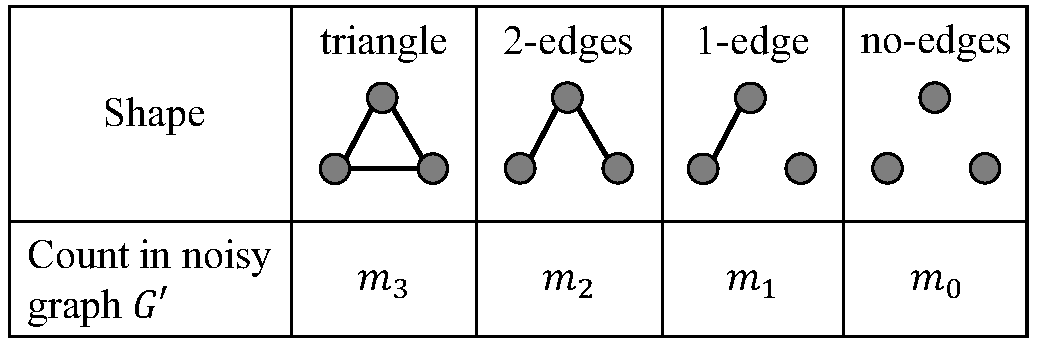
\includegraphics[width=0.9\linewidth]{fig/triplet_shape.pdf}
\vspace{-4mm}
\caption{Four types of subgraphs with three nodes.}
\label{chap1-fig:triplet_shape}
\end{figure}

Through 
% some 
% a 
clever post-processing 
% method 
known as 
% an 
empirical estimation 
% method~
\cite{Kairouz_ICML16,Murakami_USENIX19,Wang_USENIX17},
we are able to obtain an unbiased estimate of $f_\triangle(G)$ 
% with access to just $P$. 
from $G'$. 
Specifically, a subgraph with three nodes can be divided into four types depending on the number of edges. 
Three nodes with three edges form a triangle. 
We refer to three nodes with two edges, one edge, and no edges as \textit{2-edges},  \textit{1-edge}, and  \textit{no-edges}, respectively. 
Figure~\ref{chap1-fig:triplet_shape} shows their shapes. 
% Let $m_3, m_2, m_1, m_0 \in \nnints$ be respectively the number of triangles, 2-edges, 1-edge, and no-edges in $G'$. 
% Note that $\sum_{i=0}^3 m_i = \binom{n}{3}$. 
% The expectation of 
$f_\triangle(G)$ can be expressed using $m_3$, $m_2$, $m_1$, and $m_0$ as follows:

\begin{proposition}\label{chap1-prop:triangle_emp}
  %Let $\mu = e^\epsilon$. 
  Let $G'=(V,E')$ be a noisy graph generated by applying the RR to the lower triangular part of $\bmA$.
  Let $m_3, m_2, m_1, m_0 \in \nnints$ be respectively the number of triangles, 2-edges, 1-edge, and no-edges in $G'$. 
  Then 
  \begin{align}
      %\textstyle{\mathbb{E}\left[ \frac{\mu^3}{(\mu-1)^3} m_3 - \frac{\mu^2}{(\mu-1)^3} m_2 + \frac{\mu}{(\mu-1)^3} m_1 - \frac{1}{(\mu-1)^3} m_0 \right] = f_\triangle(G).}
      \textstyle{\mathbb{E}\left[ \frac{e^{3\epsilon}}{(e^\epsilon-1)^3} m_3 \hspace{-0.5mm}-\hspace{-0.5mm} \frac{e^{2\epsilon}}{(e^\epsilon-1)^3} m_2 \hspace{-0.5mm}+\hspace{-0.5mm} \frac{e^\epsilon}{(e^\epsilon-1)^3} m_1 \hspace{-0.5mm}-\hspace{-0.5mm} \frac{1}{(e^\epsilon-1)^3} m_0 \right] \hspace{-0.5mm} = \hspace{-0.5mm} f_\triangle(G).}
      \label{chap1-eq:triangle_emp}
  \end{align}
\end{proposition}

% This significantly reduces the $l_2$ error. 
Therefore, the data collector can count $m_3$, $m_2$, $m_1$, and $m_0$ from $G'$, and calculate an unbiased estimate of $f_\triangle(G)$ by (\ref{chap1-eq:triangle_emp}). 
% Algorithm~\ref{chap1-alg:subgraph-rr} contains the precise way to do this.
In Appendix~\ref{chap1-sec:RR_emp}, we show that the $l_2$ loss is significantly reduced by this empirical estimation.

\setlength{\algomargin}{4mm}
\begin{algorithm}
  \SetAlgoLined
  \KwData{Graph $G$ 
  %described by distributed 
  represented as 
  neighbor lists $\bma_1,
    \ldots, \bma_n
  \in \{0,1\}^n$, privacy budget $\epsilon \in \nnreals$.}
  \KwResult{Private estimate of $f_\triangle(G)$.}
  \For{$i=1$ \KwTo $n$}{
    %$R_i \leftarrow (RR_{\epsilon}(a_i^1), \ldots, RR_{\epsilon}(a_i^{i-1}))$\;
    $R_i \leftarrow (RR_{\epsilon}(a_{i,1}), \ldots, RR_{\epsilon}(a_{i,i-1}))$\;
    $release(R_i)$\;
  }
  %$G' \leftarrow \texttt{UndirectedGraph}(R_1, \ldots, R_{i-1})$\;
  $G'=(V,E') \leftarrow \texttt{UndirectedGraph}(R_1, \ldots, R_n)$\;
  %\tcc{Counts $T_3,T_2,T_1,T_0$ in $P$.}
  \tcc{Counts $m_3,m_2,m_1,m_0$ in $G'$.}
  %$\hat{\textbf{m}} \leftarrow \texttt{CountSubgraphs}(G',3)$\;
  $(m_3, m_2, m_1, m_0) \leftarrow \texttt{Count}(G')$\;
  %$\mu \leftarrow e^\epsilon$\;
  %\KwRet{$\frac{1}{(\mu-1)^3}(\mu^3 m_3 -\mu^2 m_2 + \mu m_1 - m_0)$}
  \KwRet{$\frac{1}{(e^\epsilon-1)^3}(e^{3\epsilon} m_3 - e^{2\epsilon} m_2 + e^\epsilon m_1 - m_0)$}

  %\caption{CountSubgraphsRR\label{chap1-alg:subgraph-rr}}
  \caption{\alg{LocalRR$_\triangle$}\label{chap1-alg:subgraph-rr}}
\end{algorithm}

Algorithm~\ref{chap1-alg:subgraph-rr} shows this algorithm. 
In line 2, user $v_i$ applies the RR with privacy budget $\epsilon$ (denoted by $RR_\epsilon$) to $a_{i,1}, \ldots, a_{i,i-1}$ 
% (which corresponds to users $v_1, \ldots, v_{i-1}$ with smaller user IDs) 
in her neighbor list $\bma_i$, and outputs $R_i = (RR_\epsilon(a_{i,1}), \ldots, RR_\epsilon(a_{i,i-1}))$. 
In other words, we apply the RR to the lower triangular part of $\bmA$ and there is no overlap between edges sent by users. 
In line 5, the data collector uses a function (denoted by \texttt{UndirectedGraph}) 
that converts the bits of $(R_1, \ldots, R_n)$ into an undirected graph $G'
= (V, E')$ by adding edge $(v_i,v_j)$ with $i>j$ to $E'$ if and only if the $j$-th bit of
$R_i$ is $1$. 
Note that $G'$ is biased, as explained above. 
In line 6, the data collector uses a function (denoted by 
\texttt{Count}) that calculates $m_3$, $m_2$, $m_1$, and $m_0$ from $G'$. 
Finally, the data collector outputs the expression inside the expectation on
the left-hand side of (\ref{chap1-eq:triangle_emp}), which is an unbiased estimator for 
$f_\triangle(G)$ by Proposition~\ref{chap1-prop:triangle_emp}.
We denote this algorithm by \alg{LocalRR$_\triangle$}.

% One subtlety of Algorithm~\ref{chap1-alg:subgraph-rr} is that, since each edge is known by two users, releasing users' edges through the RR may result in disagreements over the noisy edges. User $i$ may claim that he is
% connected to $j$, and user $j$ may claim he is not connected to $i$. 
% To avoid this problem, we assume an ordering on users, and we let user $i$ ignore edge
% $(i,j)$ if $i<j$. This means each edge is the responsibility of just one user.
% Because edge $(i,j)$ is released by user $\max\{i,j\}$, it is technically a
% directed edge. Thus, we let $P$ be the undirected graph formed by taking the
% direction out of all noisy edges released (Line 5).


\smallskip
\noindent{\textbf{Theoretical properties.}}~~\alg{LocalRR$_\triangle$} 
% Algorithm~\ref{chap1-alg:subgraph-rr} 
provides the following guarantee.

\begin{theorem}\label{chap1-thm:subgraph-rr_LDP}
  \alg{LocalRR$_\triangle$} provides $\epsilon$-edge LDP and $\epsilon$-relationship DP.
\end{theorem}

\alg{LocalRR$_\triangle$} does not have the doubling issue (i.e., it provides not $2\epsilon$ but $\epsilon$-relationship DP), because we apply the RR to the lower triangular part of $\bmA$, as explained in Section~\ref{chap1-sub:LDP}.

Unlike the RR and empirical estimation for tabular data \cite{Kairouz_ICML16}, the expected $l_2$ loss of \alg{LocalRR$_\triangle$} is complicated. 
% due to the fact that multiple triangles can involve the same edge. 
To simplify the utility analysis, we assume that $G$ is generated from the Erd\"os-R\'enyi graph distribution $\bmG(n,\alpha)$ with edge existence probability $\alpha$; i.e., each edge in $G$ with $n$ nodes is independently generated with probability $\alpha \in [0,1]$.
% which generates $G=(V,E)$ with $|V|=n$ with

\begin{theorem}\label{chap1-thm:subgraph-rr}
  Let $\bmG(n,\alpha)$ be the Erd\"os-R\'enyi graph distribution with edge existence probability $\alpha \in [0,1]$. 
  Let $p = \frac{1}{e^\epsilon+1}$ and 
  $\beta = \alpha(1-p) + (1-\alpha)p$. 
  Let 
  %$A(G, \epsilon)$ 
  $\hf_{\triangle}(G, \epsilon)$ 
  be the output of 
  %Algorithm~\ref{chap1-alg:subgraph-rr}.
  \alg{LocalRR$_\triangle$}.
  %Suppose 
  %$G \sim \bmG(n,\frac{d_{max}}{n})$, 
  If 
  $G \sim \bmG(n,\alpha)$, 
  %the Erd\"os-R\'enyi graph
  %distribution with parameter $\frac{d_{max}}{n}$.  Then, 
  then for all 
  $\epsilon \in \nnreals$, 
  %$l_2^2(A(G,\epsilon),
  $\mathbb{E}[l_2^2(\hf_{\triangle}(G, \epsilon),
  f_\triangle(G))] = 
  %O(\frac{e^{6\epsilon}}{(e^\epsilon-1)^6}d_{max}n^3)$.
  O\left(\frac{e^{6\epsilon}}{(e^\epsilon-1)^6}\beta n^4\right)$.
  %Furthermore, Algorithm~\ref{chap1-alg:subgraph-rr} provides $\epsilon$-edge LDP.
\end{theorem}

% Note that Theorem~\ref{chap1-thm:subgraph-rr} is a statement about the expected 
% % average $l_2^2$ error
% $l_2$ loss 
% over graphs 
% % $G \sim \bmG(n,\frac{d_{max}}{n})$. 
% $G \sim \bmG(n,\alpha)$. 
% This is less ideal than the case of
% Theorem~\ref{chap1-thm:k-stars} which upper bounds the 
% % $l_2^2$ error 
% $l_2$ loss for all $G \in \calG$. 
% However, 
% % $\textbf{G}(n,\frac{d_{max}}{n})$ 
% $\textbf{G}(n,\alpha)$ 
% is considered a realistic model from which
% graphs of max degree $d_{max}$ are drawn, so Theorem~\ref{chap1-thm:subgraph-rr} is
% still 
% % a strong bound.
% valid. 

Note that we assume the Erd\"os-R\'enyi model only for the utility analysis of \alg{LocalRR$_\triangle$}, and do not assume this model for the other algorithms. 
The upper-bound of \alg{LocalRR$_\triangle$} in Theorem~\ref{chap1-thm:subgraph-rr} is less ideal than the upper-bounds of the other algorithms in that it does not consider all possible graphs $G \in \calG$. 
Nevertheless, we also show that the $l_2$ loss of \alg{LocalRR$_\triangle$} is roughly consistent with Theorem~\ref{chap1-thm:subgraph-rr} in our experiments using two real datasets (Section~\ref{chap1-sec:experiments}) and 
% artificial graphs based on 
the Barab\'{a}si-Albert graphs \cite{NetworkScience}, which have power-law degree distribution (Appendix~\ref{chap1-sec:BAGraph}). 

% The parameter $\alpha$ is very small in a sparse graph. 
% For example, it is reasonable to assume that $\alpha \leq \frac{d_{max}}{n} \ll 1$. 
% On the other hand, $\beta$ is a parameter in 
The parameters $\alpha$ and $\beta$ are edge existence probabilities in the original graph $G$ and noisy graph $G'$, respectively. 
Although $\alpha$ is very small in a sparse graph, $\beta$ can be large for small $\epsilon$. 
For example, if $\alpha \approx 0$ and $\epsilon=1$, then $\beta \approx \frac{1}{e+1} = 0.27$. 
% In this case, the expected $l_2$ loss of \alg{LocalRR$_\triangle$} can be expressed as: $O\left(\frac{e^{6\epsilon}}{(e^\epsilon-1)^6}d_{max} n^3\right)$.

Theorem~\ref{chap1-thm:subgraph-rr} states that for large $n$, the $l_2$ loss of \alg{LocalRR$_\triangle$} 
($=O(n^4)$) 
% ($=O(d_{max}n^3)$) 
is much larger than the $l_2$ loss of \alg{LocalRR$_k\star$} ($=O(n)$). 
This follows from the fact that user $v_i$ 
% cannot see any edge $(v_j, v_k) \in E$ in graph $G$ and 
is not aware of any triangle formed by $(v_i, v_j, v_k)$, as explained above. 

In contrast, counting $f_\triangle(G)$ in the centralized model is much easier because the data collector sees all triangles in $G$; i.e., the data collector knows $f_\triangle(G)$. 
% After we perform graph projection 
% \cite{Day_SIGMOD16,Kasiviswanathan_TCC13,Raskhodnikova_arXiv15} 
% so that each user's degree does not exceed $\td_{max}$, 
% the 
The 
% local 
% global 
sensitivity of $f_\triangle$ 
% becomes 
is 
at most $\td_{max}$ (after graph projection). 
% Therefore, as with $k$-stars, 
Thus, 
we can consider a simple algorithm that 
% performs graph projection so that each user's degree never exceeds $\td_{max}$, 
% and then 
% adds the Laplacian noise $\Lap(\td_{max}/\epsilon)$ 
% ($\td_{max} > d_{max}$) 
% to $f_{\triangle}(G)$, and 
outputs $f_{\triangle}(G) + \Lap(\td_{max}/\epsilon)$. 
We denote this algorithm by \alg{CentralLap$_{\triangle}$}. 
\alg{CentralLap$_{\triangle}$} attains the expected $l_2$ loss ($=$ variance) of $O\left(\frac{\td_{max}^2}{\epsilon^2}\right)$. 

% \colorB{In Section~\ref{chap1-sub:two_rounds}, we propose a two-rounds LDP algorithm for triangles to significantly reduce the $l_2$ loss in the local model.}

% In Algorithm~\ref{chap1-alg:subgraph-rr}, 
The large $l_2$ loss of \alg{LocalRR$_\triangle$} is caused by the fact that 
each edge is released independently with
some probability of being flipped. 
% Thus, 
In other words, 
there are three independent random
variables that influence 
% any subgraph of size $3$ in $P$. 
any triangle in $G'$. 
The next algorithm,
using interaction, 
% is able to reduce 
reduces 
this influencing number 
% to two, 
from three to one 
% because 
% a single 
by using the fact that 
a user 
% always 
knows 
% two edges of a subgraph of size 3.
the existence of two edges for any triangle that involves the user. 

% \ji{Can we combine the last and third-last paragraphs of this section?}
% \tm{It's a little bit difficult to me because 
% the explanation is in the order of ``Thm 4 --> one-round local (third-last) --> centralized (second-last) --> two-round local (last) (--> Sec 4.3)''. Instead, I shortened the third-last paragraph.}

% \subsection{Two-Rounds LDP Algorithms for Triangles}
\subsection{Two-Rounds Algorithms for Triangles}
% \colorB{Sequentially Interactive Graph LDP Algorithms}}
\label{chap1-sub:two_rounds}

\noindent{\textbf{Algorithm.}}~~Allowing for 
% sequential interaction, 
two-rounds interaction, 
we are able to compute $f_{\triangle}$ with
a significantly improved $l_2$ loss, albeit with a higher per-user
communication overhead.
As described in Section~\ref{chap1-sub:non-interactive_triangles}, it is impossible for user $v_i$ to see edge $(v_j, v_k) \in E$ in graph $G=(V,E)$ at the first round. 
However, if 
% each user $v_i$ applies the RR to her neighbor list $\bma_i$ as in \alg{LocalRR$_\triangle$} and 
the data collector publishes a noisy graph $G'=(V,E')$ calculated by \alg{LocalRR$_\triangle$} at the first round, then 
user $v_i$ can see a noisy edge $(v_j, v_k) \in E'$ in the noisy graph $G'$ at the second round. 
Then user $v_i$ can count the number of \textit{noisy triangles} formed by
$(v_i, v_j, v_k)$ such that $(v_i,v_j) \in E$, $(v_i,v_k) \in E$, and $(v_j,v_k)
\in E'$, and send the noisy triangle counts with the Laplacian noise to the data
collector in an analogous way to \alg{LocalLap$_{k\star}$}.
Since user $v_i$ always knows that two edges $(v_i,v_j)$ and $(v_i,v_k)$ exist in $G$, 
there is only one noisy edge in any noisy triangle 
(whereas all edges are noisy in \alg{LocalRR$_\triangle$}).
% edge $(v_j,v_k)$
% random variable 
% that influences the existence of the triangle $(v_i, v_j, v_k)$ in $G$. 
This is an intuition behind our proposed two-rounds algorithm. 

As with the RR in Section~\ref{chap1-sub:non-interactive_triangles}, simply counting the noisy triangles can introduce a bias. 
Therefore, we calculate an empirical estimate of $f_\triangle(G)$ from the noisy triangle counts. 
Specifically, 
% we calculate the expectation of 
the following is the empirical estimate of $f_\triangle(G)$: 
% can be expressed as follows:
% Specifically, assume that the data collector publishes a noisy graph $G'=(V,E')$ calculated by \alg{LocalRR$_\triangle$} with privacy budget $\epsilon_0 \in \nnreals$ at the first round. 
% Let $t_i \in \nnints$ be the number of triplets $(v_i, v_j, v_k)$ such that $j < i < k$, $(v_i,v_j) \in E$, $(v_i,v_k) \in E$, and $(v_j,v_k) \in E'$; i.e., 
% the number of noisy triangles user $v_i$ can see at the second round. 
% Here we count only triplets $(v_i, v_j, v_k)$ with $j < i < k$ to avoid counting the same triplet multiple times.
% Let $s_i \in \nnints$ be the number of triplets $(v_i, v_j, v_k)$ such that $j < i < k$, $(v_i,v_j) \in E$, and $(v_i,v_k) \in E$; i.e., 
% the number of $2$-stars of which user $v_i$ is a center. 
% Then the expectation of $f_\triangle(G)$ can be calculated from $\epsilon_0$, $t_i$, and $s_i$ as follows:

\begin{proposition}\label{chap1-prop:triangle_emp_2rounds}
  Let $G'=(V,E')$ be a noisy graph generated by applying the RR with privacy budget $\epsilon_1 \in \nnreals$   to the lower triangular part of $\bmA$.
  Let $p_1 = \frac{1}{e^{\epsilon_1}+1}$. 
  Let $t_i \in \nnints$ be the number of triplets $(v_i, v_j, v_k)$ such that 
  %$j < i < k$, 
  $j < k < i$, 
  $(v_i,v_j) \in E$, $(v_i,v_k) \in E$, and $(v_j,v_k) \in E'$.
  Let $s_i \in \nnints$ be the number of triplets $(v_i, v_j, v_k)$ such that 
  %$j < i < k$, 
  $j < k < i$, 
  $(v_i,v_j) \in E$, and $(v_i,v_k) \in E$. 
  Let $w_i = t_i - p_1 s _i$. 
  Then 
  \begin{align}
      %\textstyle{\mathbb{E}[f_\triangle(G)] = \frac{1}{1-2p_1} \sum_{i=1}^n (t_i - p_1 s_i)}.
      \textstyle{\mathbb{E}\left[ \frac{1}{1-2p_1} \sum_{i=1}^n w_i \right] = f_\triangle(G).}
      \label{chap1-eq:triangle_emp_2rounds}
  \end{align}
\end{proposition}

Note that in Proposition~\ref{chap1-prop:triangle_emp_2rounds}, 
we count only triplets $(v_i, v_j, v_k)$ with 
% $j < i < k$ 
$j < k < i$ 
% to avoid counting the same triplet multiple times. 
to use only the lower triangular part of $\bmA$. 
$t_i$ is the number of noisy triangles user $v_i$ can see at the second round. 
$s_i$ is the number of $2$-stars of which user $v_i$ is a center. 
Since $t_i$ and $s_i$ can reveal information about an edge in $G$, user $v_i$ adds the Laplacian noise to $w_i$ $(= t_i - p_1 s _i)$ in (\ref{chap1-eq:triangle_emp_2rounds}), and sends it to the data collector. 
Then the data collector calculates an unbiased estimate of $f_\triangle(G)$ by (\ref{chap1-eq:triangle_emp_2rounds}). 

% Instead of releasing each edge through 
% randomized
% response, user $i$ is given a specific query depending on $P_{i-1}$, the
% subgraph of $G$ on users $1$ through $i-1$ released through randomized response.
% Like Algorithm~\ref{chap1-alg:subgraph-rr}, we assume user $i$ ignores edge $(i,j)$ if
% $i<j$. The query to user $i$ is to noisily count the number of triangles of which he is
% a part, using two of his edges and one edge in $P_{i-1}$. He releases this
% number and a randomized response on his edges so that future users may build
% $P_{i}$. 

\setlength{\algomargin}{5mm}
\begin{algorithm}
  \SetAlgoLined
  \KwData{Graph $G$ 
  %described by distributed 
  represented as 
  neighbor lists $\bma_1,
    \ldots, \bma_n
    \in \{0,1\}^n$, two privacy budgets
  %$\epsilon_0,\epsilon_1 > 0$.}
  $\epsilon_1,\epsilon_2 > 0$, $\td_{max} \in \nnints$.}
  %\KwResult{Private count of number of triangles in $G$.}
  \KwResult{Private estimate of $f_\triangle(G)$.}
  %$\rho \leftarrow \frac{1}{e^{\epsilon_0}+1}$\;
  $p_1 \leftarrow \frac{1}{e^{\epsilon_1}+1}$\;
  \tcc{First round.}
  \For{$i=1$ \KwTo $n$}{
    %$ans_i \leftarrow 0$\;
    %$R_i \leftarrow (RR_{\epsilon_0}(a_i^1), \ldots, RR_{\epsilon_0}(a_i^{i-1}))$\;
    $R_i \leftarrow (RR_{\epsilon_1}(a_{i,1}), \ldots, RR_{\epsilon_1}(a_{i,i-1}))$\;
    $release(R_i)$\;
  }
  %$P_{i-1} \leftarrow \texttt{UndirectedGraph}(R_1, \ldots, R_{i-1})$\;
  $G'=(V,E') \leftarrow \texttt{UndirectedGraph}(R_1, \ldots, R_{i-1})$\;
  \tcc{Second round.}
  \For{$i=1$ \KwTo $n$}{
    $\bma_i \leftarrow \texttt{GraphProjection}(\bma_i, \td_{max})$\;
    %$t_i \leftarrow |\{(u,v) : u,v \in [i], u<v<i, a_{i}^u = a_{i}^v = 1,(u,v) \in P_{i-1}\}|$\;
    $t_i \leftarrow |\{(v_i,v_j,v_k) : 
    %j<i<k, a_{j,i} = a_{i,k} = 1, 
    j<k<i, a_{i,j} = a_{i,k} = 1, 
    (v_j,v_k) \in E'\}|$\;
    %$s_i \leftarrow |\{(u,v) : u,v \in [i], u<v<i, a_{i}^u = a_{i}^v = 1\}|$\;
    $s_i \leftarrow |\{(v_i,v_j,v_k) : 
    %j<i<k, a_{j,i} = a_{i,k} = 1\}|$\;
    j<k<i, a_{i,j} = a_{i,k} = 1\}|$\;
    %$w_i \leftarrow t_i - \rho s_i + Lap(\frac{d_{max}(1-\rho)}{\epsilon_1})$\;
    %$w_i \leftarrow t_i - p_1 s_i + \Lap(\frac{\td_{max}(1-p_1)}{\epsilon_2})$\;
    $w_i \leftarrow t_i - p_1 s_i$\;
    $\hw_i \leftarrow w_i + \Lap(\frac{\td_{max}}{\epsilon_2})$\;
    %$release(R_i, w_i)$\;
    $release(\hw_i)$\;
  }
  %$ans \leftarrow \frac{1}{1-2\rho}\sum_{i=1}^n w_i$\;
  \KwRet{$\frac{1}{1-2p_1}\sum_{i=1}^n \hw_i$}
  %\caption{CountSubgraphsTwoRound\label{chap1-alg:subgraph-interactive}}
  \caption{\alg{Local2Rounds$_\triangle$}}\label{chap1-alg:subgraph-interactive}
\end{algorithm}

Algorithm~\ref{chap1-alg:subgraph-interactive} contains the formal
description of this process. 
It takes as input a graph $G$, 
% (represented as neighbor lists $\bma_1, \ldots, \bma_n$), 
the privacy budgets $\epsilon_1, \epsilon_2 \in \nnreals$ at the first and second rounds, respectively, 
and 
% It also takes as input 
% an upper-bound $\td_{max}$ on the maximum degree $d_{max}$ of $G$ 
a non-negative integer $\td_{max} \in \nnints$. 
% in the same way as \alg{LocalLap$_{k\star}$}. 
% We will describe the private computation of $d_{max}$ with edge LDP at the end of Section~\ref{chap1-sub:two_rounds}. 
At the first round, we 
apply the RR to the lower triangular part of $\bmA$ 
(i.e., there is no overlap between edges sent by users) 
% . 
and use the \texttt{UndirectedGraph} function to 
obtain a noisy graph $G'=(V,E')$ by the RR in the same way as Algorithm~\ref{chap1-alg:subgraph-rr}. 
Note that $G'$ is biased. 
We calculate an unbiased estimate of $f_\triangle(G)$ from $G'$ at the second round.  
% Then we use the \texttt{UndirectedGraph} function, which makes an undirected graph $G'
% = (V, E')$ by adding edge $(i,j)$ with $i>j$ to $E'$ if and only if the $j$-th bit of $R_i$ is $1$. 

At the second round, each user $v_i$ 
calculates $\hw_i = w_i + \Lap(\frac{\td_{max}}{\epsilon_2})$ 
%  and 
by adding the Laplacian noise to $w_i$ 
% $(= t_i - p_1 s _i)$, 
in Proposition~\ref{chap1-prop:triangle_emp_2rounds} 
whose 
% local 
% global 
sensitivity is at most 
% $d_{max} (1-p_1)$, 
$\td_{max}$ 
% (after graph projection), 
(as we will prove in Theorem~\ref{chap1-thm:local2rounds_LDP}). 
Finally, we output $\frac{1}{1-2p_1}\sum_{i=1}^n \hw_i$, which is an unbiased estimate of $f_\triangle(G)$ by Proposition~\ref{chap1-prop:triangle_emp_2rounds}. 
We call this algorithm \alg{Local2Rounds$_\triangle$}.

% The intuitive reason Algorihtm~\ref{chap1-alg:subgraph-interactive} performs better than 
% Algorithm~\ref{chap1-alg:subgraph-rr} is that a noisy triangle is counted using two 
% noisy computations, the noisy edge in
% $P_{i-1}$ and user $i$'s noisy count. In Algorithm~\ref{chap1-alg:subgraph-rr}, each
% subgraph of size $3$ in $P$ is the result of three noisy computations.

\smallskip
\noindent{\textbf{Theoretical properties.}}~~\alg{Local2Rounds$_\triangle$} 
% Algorithm~\ref{chap1-alg:subgraph-interactive} 
has the following 
% performance 
guarantee.

\begin{theorem}\label{chap1-thm:local2rounds_LDP}
  %If the maximum degree $d_{max}$ of $G$ is at most $\td_{max}$, 
  \alg{Local2Rounds$_\triangle$}
  provides $(\epsilon_1 + \epsilon_2)$-edge LDP and $(\epsilon_1 + \epsilon_2)$-relationship DP.
\end{theorem}

As with \alg{LocalRR$_\triangle$}, \alg{Local2Rounds$_\triangle$} does not have the doubling issue; i.e., it provides $\epsilon$-relationship DP (not $2\epsilon$). 
This follows from the fact that we 
use only the lower triangular part of $\bmA$; 
% count each triplet $(v_i,v_j,v_k)$ only once; 
i.e., we assume 
%$j<i<k$ 
$j<k<i$ 
in counting $t_i$ and $s_i$. 

\begin{theorem}\label{chap1-thm:local2rounds}
  Let 
  %$A(G, d_{max}, \epsilon_0, \epsilon_1)$ 
  $\hf_{\triangle}(G, \epsilon_1, \epsilon_2, \td_{max})$ 
  be the output of 
  %Algorithm~\ref{chap1-alg:subgraph-interactive}. 
%   \alg{LocalRR$_\triangle$}. 
  \alg{Local2Rounds$_\triangle$}. 
  Then, for all 
  %$d_{max} \in \nats$,
  $\epsilon_1,\epsilon_2 \in \nnreals$, 
  $\td_{max} \in \nnints$,
  and $G\in \calG$ such that the
  maximum degree $d_{max}$ of $G$ is 
  at most 
  $\td_{max}$,
  %$l_2^2(A(G,d_{max},\epsilon_0,\epsilon_1) 
  $\mathbb{E}[l_2^2(\hf_{\triangle}(G, \epsilon_1, \epsilon_2, \td_{max}), f_\triangle(G))] 
  \leq
    O\left(\frac{e^{\epsilon_1}}{(1-e^{\epsilon_1})^2} \left(\td_{max}^3 n +
    \frac{e^{\epsilon_1}}{\epsilon_2^2}\td_{max}^2 n\right)\right)$.
\end{theorem}

Theorem~\ref{chap1-thm:local2rounds} means that for triangles, the $l_2$ loss 
% of \alg{LocalRR_$\triangle$} 
is reduced from $O(n^4)$ to $O(\td_{max}^3n)$ by introducing an additional round. 

% The upper and lower bounds on the $l_2$ losses for the central,
% % local non-interactive, 
% one-round local, 
% and 
% % local sequentially interactive 
% two-rounds local 
% models discussed in
% this section appear in Table~\ref{chap1-tab:perf}.

\smallskip
\noindent{\textbf{Private calculation of $d_{max}$.}}~~As with $k$-stars, we can privately calculate $d_{max}$ 
% with edge LDP 
by using the method described in Section~\ref{chap1-sub:non-interactive_k_stars}. 
Furthermore, the private calculation of $d_{max}$ does not increase the number of rounds; i.e., we can run \alg{Local2Rounds$_\triangle$} with the private calculation of $d_{max}$ in two rounds. 

Specifically, let $\epsilon_0 \in \nnreals$ be the privacy budget for the private calculation of $d_{max}$. 
At the first round, each user $v_i$ adds $\Lap(\frac{1}{\epsilon_0})$ to her degree $d_i$, 
% (i.e., number of ``$1$''s in her neighbor list $\bma_i$), 
and sends the noisy degree $\hd_i$ ($=d_i + \Lap(\frac{1}{\epsilon_0})$) to the data collector, along with the outputs $R_i = (RR_\epsilon(a_{i,1}), \ldots, RR_\epsilon(a_{i,i-1}))$ of the RR. 
The data collector calculates the noisy max degree $\hd_{max}$ ($= \max\{\hd_1,
\ldots, \hd_n\}$) as an estimate of $d_{max}$, and sends it back to all users. 
At the second round, we run \alg{Local2Rounds$_\triangle$} with input $G$ (represented as $\bma_1, \ldots, \bma_n$), $\epsilon_1$, $\epsilon_2$, and $\lfloor \hd_{max} \rfloor$. 

% At the second round, each user performs graph projection; i.e., if $d_i$ exceeds $\hd_{max}$, user $v_i$ randomly selects $\hd_{max}$ neighbors from her neighbor list $\bma_i$ (otherwise, user $v_i$ uses $\bma_i$ as it is). 
% Let $\bma'_i \in \{0,1\}^n$ be a neighbor list of user $v_i$ after this projection. 
% We run the second round part (lines $7$ to $12$) of \alg{Local2Rounds$_\triangle$} with input $\bma'_1, \ldots, \bma'_n$, $\epsilon_1$, $\epsilon_2$, 
% and $\hd_{max}$. 

At the first round, the calculation of $\hd_{max}$ provides $\epsilon_0$-edge LDP. 
% because each user's degree has the sensitivity $1$ under edge LDP. 
Note that it provides $2\epsilon_0$-relationship DP (i.e., it has the doubling issue) because one edge $(v_i,v_j) \in E$ affects both of the degrees $d_i$ and $d_j$ by 1. 
At the second round, \alg{LocalLap$_{k\star}$} provides $(\epsilon_1 + \epsilon_2)$-edge LDP and 
$(\epsilon_1 + \epsilon_2)$-relationship DP (Theorem~\ref{chap1-thm:local2rounds_LDP}). 
% because each user $v_i$'s degree in $\bma'_i$ never exceeds $\hd_{max}$. 
% (and then Theorem~\ref{chap1-thm:local2rounds_LDP} holds). 
Then by the composition theorem~\cite{DP}, this two-rounds algorithm provides $(\epsilon_0 + \epsilon_1 + \epsilon_2)$-edge LDP and $(2\epsilon_0 + \epsilon_1 + \epsilon_2)$-relationship DP. 
Although the total privacy budget is larger for relationship DP, the difference ($=\epsilon_0$) can be very small. 
In fact, we set $(\epsilon_0, \epsilon_1, \epsilon_2) = (0.1, 0.45, 0.45)$ or $(0.2, 0.9, 0.9)$ in our experiments (i.e., the difference is $0.1$ or $0.2$), and show that this algorithm provides almost the same utility as \alg{Local2Rounds$_\triangle$} with the true max degree $d_{max}$. 

\smallskip
\noindent{\textbf{Time complexity.}}~~We also note that \alg{Local2Rounds$_\triangle$} has an advantage over \alg{LocalRR$_\triangle$} in terms of the time complexity. 
% in addition to the expected $l_2$ loss. 

Specifically, \alg{LocalRR$_\triangle$} is inefficient because the data collector has to count the number of triangles $m_3$ in the noisy graph $G'$. 
Since the noisy graph $G'$ is dense (especially when $\epsilon$ is small) and there are $\binom{n}{3}$ subgraphs with three nodes in $G'$, the number of triangles is $m_3 = O(n^3)$. 
Then, the time complexity of \alg{LocalRR$_\triangle$} is 
% $O(n)$ for each user's part and $O(n^3)$ for the data collector's part, 
also $O(n^3)$, which is not practical for a graph with a large number of users $n$.
In fact, we implemented \alg{LocalRR$_\triangle$} ($\epsilon=1$) with C/C++ and measured its running time using one node of a supercomputer (ABCI: AI Bridging Cloud Infrastructure \cite{ABCI}). 
When $n=5000$, $10000$, $20000$, and $40000$, the running time was $138$, $1107$, $9345$, and $99561$ seconds, respectively; i.e., the running time was almost cubic in $n$. 
We can also estimate the running time for larger $n$. 
For example, when $n=1000000$, \alg{LocalRR$_\triangle$} ($\epsilon=1$) would require about $35$ years $(=1107 \times 100^3 /(3600 \times 24 \times 365))$. 
% Even if we use $1000$ nodes of the supercomputer (the ABCI has $1088$ nodes \cite{ABCI}) in parallel, \alg{LocalRR$_\triangle$} would require over $10$ days. 

In contrast, the time complexity of \alg{Local2Rounds$_\triangle$} 
% for each user 
is 
% $O(n)$ in the first round (l.3-4 in Algorithm~\ref{chap1-alg:subgraph-interactive}) and $O(d_{max}^2)$ in the second round (l.8-13 in Algorithm~\ref{chap1-alg:subgraph-interactive})). 
% $O(n + d_{max}^2)$ for each user's part and $O(n)$ for the data collector's part at the second round. 
$O(n^2 + n d_{max}^2)$\footnote{When we 
% want to 
evaluate 
% the utility of 
\alg{Local2Rounds$_\triangle$} in our experiments, 
% When we evaluate the utility of \alg{Local2Rounds$_\triangle$} on one computer, 
we can apply the RR to only edges that are required at the second round; i.e., $(v_j,v_k) \in G'$ in line 8 of Algorithm~\ref{chap1-alg:subgraph-interactive}. 
Then the time complexity of \alg{Local2Rounds$_\triangle$} 
% is 
can be reduced to 
$O(n d_{max}^2)$ in total. 
We also confirmed that when $n=1000000$, the running time of \alg{Local2Rounds$_\triangle$} was $311$ seconds on one node of the ABCI. 
% , which is $3.5 \times 10^6$ times faster than \alg{LocalRR$_\triangle$}. 
Note, however, that this does \textit{not} protect individual privacy, because it reveals the fact that users $v_j$ and $v_k$ are friends with $u_i$ to the data collector.}. 
% including the private calculation of $d_{max}$. 
The factor of $n^2$ comes from the fact that the size of the noisy graph $G'$ is $O(n^2)$. 
This also causes a large communication overhead, as explained below.
% Further reduction of the time complexity by compressing the graph size (e.g., via graph projection) is left for future work.}

\smallskip
\noindent{\textbf{Communication overhead.}}~~In 
% The \alg{Local2Rounds$_\triangle$} has a quadratic communication overhead.
\alg{Local2Rounds$_\triangle$}, each user need to see the noisy graph $G'$ 
of size $O(n^2)$ 
% with $O(n^2)$ bits 
to count $t_i$ and $s_i$. 
% must count $t_i$ and $s_i$ which depend on $G'$, the private graph computed in the first round. 
% Thus, each user must see $G'$, a graph with $O(n^2)$ bits. 
This results in a per-user communication overhead of $O(n^2)$. 
% We 
Although we 
do not simulate the communication overhead in our experiments that use \alg{Local2Rounds$_\triangle$}, 
% but 
the $O(n^2)$ overhead 
% would 
might 
limit its application in very large graphs. 
An interesting avenue of future work is how to compress the graph size (e.g., via graph projection or random projection) to reduce both the time complexity and the communication overhead.
% Again, compressing the graph size (e.g., via graph projection) is left for future work.

\begin{table*}
  \centering
\begin{tabular}{|l|l|l|l|l|l|l|}
  \hline
  & Centralized & \spantwo{One-round local} & Two-rounds local \\
  \hline
  & Upper Bound & Lower Bound & Upper Bound & Upper Bound \\ \hline

  $f_{k\star}$
  & $O\left( \frac{d_{max}^{2k-2}}{\epsilon^2} \right)$  
  &  $\Omega\left( \frac{e^{2\epsilon}}{(e^{2\epsilon}+1)^2}d_{max}^{2k-2}n \right)$ 
  &  $O\left( \frac{d_{max}^{2k-2}}{\epsilon^2}n \right)$ 
  &  $O\left( \frac{d_{max}^{2k-2}}{\epsilon^2}n \right)$ \\ \hline

 $f_\triangle$ 
  &  $O\left(\frac{d_{max}^2}{\epsilon^2}\right)$ 
  &  $\Omega\left( \frac{e^{2\epsilon}}{(e^{2\epsilon}+1)^2}d_{max}^2n \right)$
  &  $O\left(\frac{e^{6\epsilon}}{(e^{\epsilon}-1)^6}n^4\right)$ 
  (when $G \sim \bmG(n,\alpha)$)
  %(randomized bound)
  &  $O\left(\frac{e^\epsilon}{(e^\epsilon-1)^2}(d_{max}^3 n +
  \frac{e^\epsilon}{\epsilon^2}d_{max}^2 n)\right)$ \\ \hline

\end{tabular}
% \vspace{-3.5mm}
\vspace{-2mm}
\caption{Bounds on $l_2$ losses for privately estimating $f_{k\star}$ and
$f_{\triangle}$ with $\epsilon$-edge LDP. For upper-bounds, we assume that  $\td_{max}=d_{max}$. 
For the centralized model, we use the Laplace mechanism. For
the one-round $f_\triangle$ algorithm, we apply Theorem~\ref{chap1-thm:subgraph-rr} 
with constant $\alpha$. For the two-round protocol $f_\triangle$ algorithm, we
apply Theorem~\ref{chap1-thm:local2rounds} with
$\epsilon_1=\epsilon_2=\frac{\epsilon}{2}$. }\label{chap1-tab:perf}
\end{table*}

\subsection{Lower Bounds}
\label{chap1-sub:lower_bounds}

We show a general lower bound on the $l_2$ loss of private estimators $\hat{f}$ of
real-valued functions $f$ in the one-round LDP model. Treating $\epsilon$ as a
constant, we have shown that 
when $\td_{max}=d_{max}$, 
% for graphs $G$ of maximum degree $d_{max}$,
the expected $l_2$ loss of \alg{LocalLaplace$_{k\star}$} is 
% $l_2^2(\alg{LocalLaplace$_{k\star}$}(G), f_{k\star}(G)) = 
$O(nd_{max}^{2k-2})$
(Theorem~\ref{chap1-thm:k-stars}). 
% and 
% the expected $l_2$ loss of 
% \alg{Local2Rounds$_\triangle$} is 
% \alg{LocalRR$_\triangle$} is 
%$l_2^2(\alg{LocalRR$_\triangle$}(G),
% f_{k\star}(G) ) = 
% $O(nd_{max}^2)$ 
% $O(nd_{max}^3)$ 
% $O(n^4)$ 
% (Theorem~\ref{chap1-thm:local2rounds}). 
% (Theorem~\ref{chap1-thm:subgraph-rr}). 
However, in
the centralized 
% edge-DP 
model, we can use
the Laplace mechanism with sensitivity 
$2\binom{d_{max}}{k-1}$ 
% and 
%$d_{max}^2$,
% $d_{max}$ 
% respectively, 
to obtain $l_2^2$ errors of $O(d_{max}^{2k-2})$ 
% and
% $O(d_{max}^2)$, respectively 
for $f_{k\star}$. 
% and $f_\triangle$. 
Thus, we ask
if 
% the factors of $n$ are 
the factor of $n$ is 
necessary 
% in the local model. 
in the one-round LDP model.

We 
% partially 
answer this question affirmatively.
We show for many types of queries $f$, there is a lower bound on 
% $l_2^2(f(\bmA), \hf(\bmA))$ 
$l_2^2(f(G), \hf(G))$ 
for any private estimator $\hf$ of the form
\begin{equation}\label{chap1-eq:one-round-lower}
%   \hf(\bmA) = \tilde{f}(\calR_1(\bma_1), \ldots, \calR_n(\bma_n)).
  \hf(G) = \tilde{f}(\calR_1(\bma_1), \ldots, \calR_n(\bma_n)),
\end{equation}
where 
$\calR_1, \ldots, \calR_n$ satisfy 
% $\epsilon$-relationship or $\epsilon$-edge DP 
$\epsilon$-edge LDP or $\epsilon$-relationship DP 
and $\tilde{f}$ is an aggregate function that takes $\calR_1(\bma_1), \ldots, \calR_n(\bma_n)$ as input and outputs $\hf(G)$. 
Here we assume that $\calR_1, \ldots, \calR_n$ 
% and 
are independently run, meaning that they are in the one-round
setting.
% 
% Our lower bound has the form of $\Omega(nD^2)$, where $D$ is a positive real
% number depending on $f$ that is similar to, but stronger than, the global sensitivity $GS_f$.
% Global sensitivity by itself cannot provide a strong lower bound in the
% local model. As a counterexample, if $f$ were the function that is always $0$ or $GS_f$,
% then an estimator $\hf$ that predicts $0$ would satisfy
% $l_2^2(f(\bmA),\hf(\bmA)) = O(GS_f^2)$
% for all adjacency matrices $\bmA$. 
% 
% Instead, we 
For our 
%this 
lower bound,
% we consider $f$ to be a function on graphs. 
% not matrices. 
% Then 
% We 
we 
require 
that 
input edges to $f$ 
% to 
be ``independent'' in the sense that 
% and 
adding an edge to an input graph $G$  
independently 
% increase 
change 
$f$ by at least $D \in \reals$. 
% over a set of input graphs. 
% Notice that we consider $f$ to be a function on graphs, not
% matrices, for this lower bound. 
The specific structure of input graphs we require is as follows:

\begin{definition}\label{chap1-def:mono-cube}[$(n,D)$-independent cube for $f$]
  Let 
  %$D \in \reals$. 
  $D \in \nnreals$. 
  For 
  %$k \in \nats$, 
  $\kappa \in \nats$, 
  let $G=(V,E) \in \calG$ be a graph on 
  %$n = 2k$ 
  $n = 2\kappa$ 
  nodes, and let 
  %$M = \{(v_{i_1}, v_{i_2}),(v_{i_3},v_{i_4}),\ldots,(v_{i_{2k-1}},v_{i_{2k}})\}$ 
  $M = \{(v_{i_1}, v_{i_2}),(v_{i_3},v_{i_4}),\ldots,(v_{i_{2k-1}},v_{i_{2\kappa}})\}$ 
  for integers $i_j \in [n]$ 
  %denote 
  be 
  a set of edges such that each of $i_1, \ldots, i_{2\kappa}$ is distinct (i.e., perfect matching on the nodes).
%   a perfect
%   matching on the 
%   nodes, 
%   meaning each 
%   of $i_1, \ldots, i_{2k}$ 
%   is distinct. 
  %Furthermore,
  Suppose that 
  %the perfect matching 
  $M$ is disjoint from 
  $E$; 
  %$G$; 
  i.e., 
  % , meaning 
  %$(v_{i_{2j-1}}, v_{i_{2j-2}}) \notin G$. 
  %$(v_{i_{2j-1}}, v_{i_{2j}}) \notin G$ 
  $(v_{i_{2j-1}}, v_{i_{2j}}) \notin E$ 
  for any 
  %$j\in[k]$. 
  $j\in[\kappa]$. 
  Let 
%   $\calA = \{G \cup N : N \subseteq M\}$.
  $\calA = \{(V, E \cup N): N \subseteq M\}$.
  %Notice 
  Note that 
  $\calA$ is a set of 
  %$2^k$ 
  $2^\kappa$ 
  graphs.
  We say $\calA$ 
  %defines 
  %forms 
  is 
  an \emph{$(n,D)$-independent cube for $f$} if for all
  %$G_1, G_2 \in \calA$ such that $|G_1| + 1 = |G_2|$, 
  $G'=(V,E') \in \calA$, 
  %$G \in \calA$, 
  we have
  \[
    % f(G) = f(G') + \sum_{e \in M} \textbf{1}[e \in G] C_e
    f(G') = f(G) + \sum_{e \in E' \cap M} C_e,
  \]
  where $C_e \in \reals$ satisfies $|C_e| \geq D$ for any $e \in M$.
%   for non-negative real numbers 
%   $\{C_e : e \in M, |C_e| \geq D\}$.}
%   for real numbers 
%   $\{C_e : e \in M\}$ satisfying $|C_e| \geq D$.
\end{definition}

\begin{figure}[t]
  \centering
%   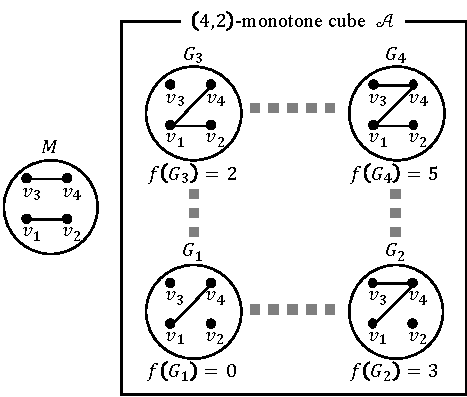
\includegraphics[width=0.88\linewidth]{fig/MonoCube.pdf}
  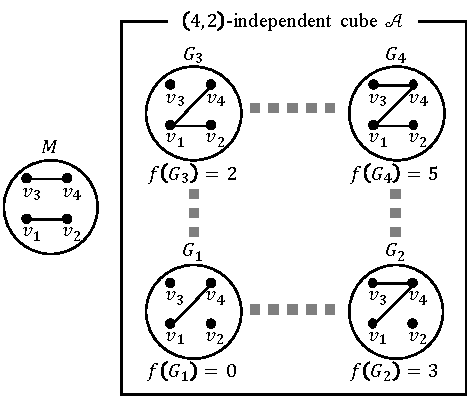
\includegraphics[width=0.9\linewidth]{fig/IndCube.pdf}
  \vspace{-2mm}
  \caption{
    $(4,2)$-independent cube $\calA$ for $f$. 
    In this example, $M = \{(v_1,v_2),(v_3,v_4)\}$, $G_1=(V,E)$, $\calA = \{(V, E \cup N): N \subseteq M\}$, 
    $C_{(v_1,v_2)}=2$, and $C_{(v_3,v_4)}=3$.
    %Definition~\ref{chap1-def:mono-cube} requires that $f$ increase by at least $D=2$ along the dotted gray lines, which it does.
    Adding $(v_1,v_2)$ and $(v_3,v_4)$ increase $f$ by $2$ and $3$, respectively.
  }\label{chap1-fig:mono-cube}
\end{figure}

\begin{figure}[t]
  \centering
  %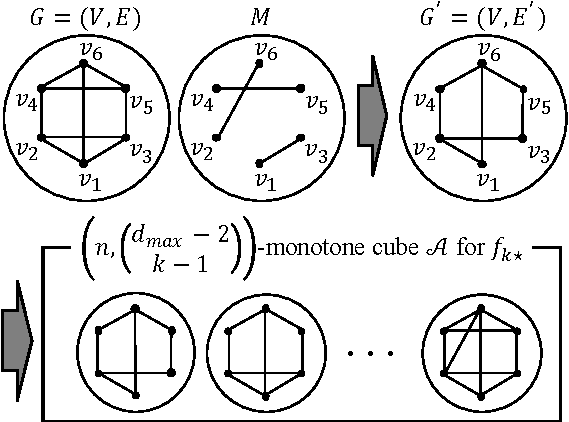
\includegraphics[width=0.88\linewidth]{fig/MonoCube_kstar.pdf}
  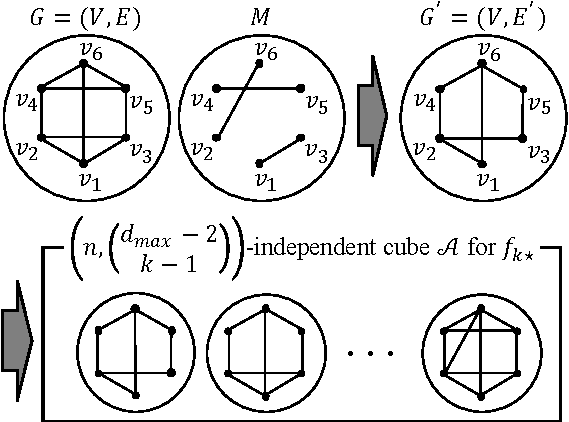
\includegraphics[width=0.9\linewidth]{fig/IndCube_kstar.pdf}
  \vspace{-2mm}
  \caption{
    Construction of an independent cube for a $k$-star function ($n=6$, $d_{max}=4$). 
    From a 
    %$(d_{max} - 1)$-
    $3$-regular graph $G=(V,E)$ and $M=\{(v_1,v_3),(v_2,v_6),(v_4,v_5)\}$, we make a graph $G'=(V,E')$ such that $E' = E \setminus M$. 
    Then $\calA = \{(V, E' \cup N): N \subseteq M\}$ forms an
    $(n, 2\binom{d_{max}-2}{k-1})$-independent cube for $f_{k\star}$.
  }\label{chap1-fig:mono-cube_kstar}
\end{figure}

% We show how to construct an $(n, \binom{d_{max}-3}{k-1})$ monotone cube
% $\mathcal{A}_{k\star}$ for
% $f_{k\star}$. First, we have to take care of a technicality.
% Note that $f_{k\star}(\bmA)$ only operates on symmetric graphs. We extend it to 
% general graphs in a natural way: let $f_{k\star}^{ext}(\bmA)$
% count the number of pointed-out $k$-stars in $\bmA$. Let
% $sym(\mathcal{A})$ be only those matrices in $\mathcal{A}$ that are symmetric,
% corresponding to undirected graphs. We show in the Appendix
% that if $\hf$ privately estimates $f_{k\star}^{ext}$ in the one-round
% edge LDP model, then there is a private estimator $\hat{g}$ that estimates
% $f_{k\star}$ in the one-round edge-LDP model such that
% \begin{multline}\label{chap1-eq:sym-lower-bound}
%   \E_{\bmA \sim U(\mathcal{A}_{k\star})}[l_2^2(f^{ext}_{k\star}(\bmA),
%   \hf(\bmA))] \\ \leq 
%   \E_{\bmA \sim U(sym(\mathcal{A}_{k\star}))} [l_2^2(f_{k\star}(\bmA),
%   \hf(\bmA))] + O(D^2)
% \end{multline}

Such a set of inputs has an ``independence'' property because,
regardless of which edges from $M$ has been added before, adding edge $e \in M$
always changes $f$ by $C_e$. 
Figure~\ref{chap1-fig:mono-cube} shows an example of a $(4,2)$-independent cube for $f$. 

% For example, 
We can also construct 
% an
% Our 
% $(n,\binom{d_{max}-3}{k-1})$ 
% $(n,\binom{d_{max}-4}{k-1})$ 
a independent cube for 
a $k$-star function 
% on directed graphs 
as follows. 
% $f_{k\star}^{ext}$ is the
% following:
% Assume $d_{max}$ and $n$ are both even. 
Assume that $n$ is even. 
It is well known in graph theory that if $n$ is even, then 
for any $d\in[n-1]$, there exists a 
$d$-regular graph where every node has degree $d$ \cite{Ganesan_arXiv18}. 
%Assume $n$ and $d_{max}$ are even and 
Therefore, there exists a 
% Let $G \in \calG$ be a $(d_{max}-1)$-regular graph 
$(d_{max}-1)$-regular graph $G=(V,E)$ 
of size $n$. 
% or a graph 
% in which every node has degree $d_{max}-1$. 
% It is a standard result in graph theory that 
% for any $d\in[n-1]$, 
% $d$-regular graphs exist 
% % for all $d$ 
% when $n$ is even.
Pick an arbitrary perfect matching $M$ on the nodes. Now, let 
% $G' = G \setminus M$. 
$G' = (V,E')$ such that $E' = E \setminus M$. 
Every node in $G'$ has degree between $d_{max}-2$ and $d_{max}-1$. 
Adding an edge in $M$ to $G'$ will produce at least
$2\binom{d_{max}-2}{k-1}$ new $k$-stars.
%the resulting graph be $\bmA = \{\bma_1,\ldots, \bma_n\}$.
%The collection $\prod_{i=1}^n \{\bma_i, \bma_i'\}$ (where the product is the Cartesian product) 
%forms an
% $(n,\binom{d_{max}-3}{k-1})$ 
% $(n,\binom{d_{max}-4}{k-1})$ 
Thus, $\calA = \{(V, E' \cup N): 
% G' \cup N : 
N \subseteq M\}$ forms an
$(n, 2\binom{d_{max}-2}{k-1})$-independent cube for $f_{k\star}$. 
% for $f_\triangle^{ext}$ 
% $\binom{d_{max}-3}{k-1}$ 
% $\binom{d_{max}-4}{k-1}$ 
%Similarly, for even natural number $l \in \nats$ such that $d_{max}>l+2$, we can construct an $(n,\binom{d_{max}-l-2}{k-1})$ monotone cube from the adjacency matrix of a collection of cliques of size $d_{max}-l$.
Note that the maximum degree of each graph in $\calA$ is at most $d_{max}$. 
Figure~\ref{chap1-fig:mono-cube_kstar} shows how to construct an independent cube for a $k$-star function when $n=6$ and $d_{max}=4$. 

% Let $U(\mathcal{A})$ be the uniform distribution over an $(n,D)$ monotone cube $\mathcal{A}$. 
Using the structure that the $(n,D)$-independent cube imposes on $f$,
we can prove a lower bound:
\begin{theorem}\label{chap1-thm:lower-bound}
  Let 
  %$\hf(\bmA)$ 
  $\hf(G)$ 
  have the form of~\eqref{chap1-eq:one-round-lower}, 
  where $\calR_1, \ldots, \calR_n$ are independently run.
  %Assume that 
  %$(\calR_1, \ldots, \calR_n)$ 
  %satisfy 
  %provide 
  %$\epsilon$-relationship DP. 
  %and are independently run.
  Let $\cal{A}$ be an $(n,D)$-independent cube for $f$. 
  If 
  $(\calR_1, \ldots, \calR_n)$ 
  provides 
  $\epsilon$-relationship DP, 
  then 
  %, with 
  %$\bmA$ 
  %$G$ 
  %uniformly drawn from $\calA$, 
  we have
  \[
    % \E_{\bmA, \calR_1, \ldots, \calR_n}[l_2^2(f(\bmA), \hf(\bmA))] =
    % \Omega(\frac{e^{\epsilon}}{(e^{\epsilon}+1)^2}nD^2).
    \frac{1}{\calA} \sum_{G \in \calA} \E[l_2^2(f(G), \hf(G))] =
    \Omega\left(\frac{e^{\epsilon}}{(e^{\epsilon}+1)^2}nD^2\right).
  \]
\end{theorem}

% \begin{corollary}\label{chap1-cor:lower-bound2}
%   If $\hf$ satisfies $\epsilon$-edge LDP in the one-round model, then $\E_{\bmA \sim U(\mathcal{A})}[l_2^2(f(\bmA), \hf(\bmA))] =
%   \Omega(\min\{1, \frac{e^{4\epsilon}}{(e^{4\epsilon}-1)^2}\}nD^2)$.
% \end{corollary}

A corollary of Theorem~\ref{chap1-thm:lower-bound} is that if $\calR_1, \ldots,
\calR_n$ satisfy $\epsilon$-edge LDP, then they satisfy $2\epsilon$
-relationship DP and thus for edge LDP we have a lower bound of
$\Omega\left(\frac{e^{2\epsilon}}{(e^{2\epsilon}+1)^2}nD^2\right)$.
% predictor $\hf$ predicting the average $\E_{\bmA \sim U(\mathcal{A})}[f(\bmA)]$
% will satisfy $\E_{\bmA \sim U(\mathcal{A})}[l_2^2(f(\bmA), \hf(\bmA))] =
% O(nD^2)$ regardless of $\epsilon$. To overcome this problem, one would have to 
% consider a different input structure for $f$ than the $(n,D)$ monotone cube, 
% but we leave this for future work.

Theorem~\ref{chap1-thm:lower-bound}, combined with the fact that there exists an
% $(n,\binom{d_{max}-2}{k-1})$ 
$(n,2\binom{d_{max}-2}{k-1})$-independent cube for 
a $k$-star function 
% $f_{k\star}$ 
% and~\eqref{chap1-eq:sym-lower-bound}, 
implies Corollary~\ref{chap1-cor:kstars-lb}. 
% (see Appendix~\ref{chap1-sub:proof_cor_kstars-lb} for details).
In Appendix~\ref{chap1-sub:cube_triangle}, we also construct an $(n, \frac{d_{max}}{2}-2)$
independent cube 
for $f_\triangle$ and establish a lower bound of 
$\Omega(\frac{e^{2\epsilon}}{(e^{2\epsilon}+1)^2} nd_{max}^2)$ for
$f_\triangle$. 

The upper and lower bounds on the $l_2$ losses 
% for the central,
% local non-interactive, 
% one-round local, 
% and 
% local sequentially interactive 
% two-rounds local 
% models discussed 
shown in
this section appear in Table~\ref{chap1-tab:perf}.

% %-------------------------------------------------------------------------------
\section{Theoretical Analysis}
\label{chap1-sec:theoretical}
%-------------------------------------------------------------------------------
aaa

\subsection{Lower Bounds}
\label{chap1-sub:lower_bounds}
aaa

\subsection{Upper Bounds}
\label{chap1-sub:upper_bounds}


%-------------------------------------------------------------------------------
\section{Experiments}
\label{sec:experiments}
%-------------------------------------------------------------------------------

% We conducted experiments to evaluate our proposed algorithms. 
% In particular, we 
Based on our theoretical results in Section~\ref{sec:algorithms}, we would like to pose the following questions:
\begin{itemize}
    \item For triangle counts, how much does the two-rounds interaction help over a single round in practice?
    \item What is the privacy-utility trade-off 
    %for subgraph counts in the local model 
    of our LDP algorithms 
    (i.e., how beneficial are our LDP algorithms)?
    %\item Is it possible to accurately estimate triangle counts and $k$-star counts in the local model?
\end{itemize}
We conducted experiments to answer to these questions. 

\subsection{Experimental Set-up}
\label{sub:setup}
% We conducted experiments to evaluate our proposed algorithms. 
% In our experiments, 
We used the following two large-scale datasets:

\smallskip
% \noindent{\textbf{Remark.}}~~
\noindent{\textbf{IMDB.}}~~The Internet Movie Database (denoted by \IMDB{}) 
% was used for the Graph Drawing 2005 contest 
\cite{IMDB_GD05} 
% . It 
includes a bipartite graph between $896308$ actors and $428440$ movies. 
% where an edge between an actor and a movie represents that the actor participated in the movie. 
% We assumed $896308$ actors as users ($n=896308$). 
We assumed actors as users. 
From the bipartite graph, we extracted 
% an adjacency matrix $\bmA=(a_{ij})$, where $a_{ij} = 1$ 
% a graph $G=(V,E)$ with $896308$ nodes, where node $v_i$ represents the $i$-th actor and edge $(v_i, v_j) \in E$ represents that actors $v_i$ and $v_j$ have played in the same movie. 
a graph $G^*$ with $896308$ nodes (actors), where an edge between two actors represents that they have played in the same movie. 
There are $57064358$ edges in $G^*$, and the average degree in $G^*$ is $63.7$ $(=\frac{57064358}{896308})$.

\smallskip
\noindent{\textbf{Orkut.}}~~The 
% Orkut is a social networking service operated by Google from $2004$ to $2014$. 
Orkut online social network dataset (denoted by \Orkut{})  \cite{snapnets} includes a graph $G^*$ with $3072441$ users and $117185083$ edges. 
The average degree in $G^*$ is $38.1$ $(=\frac{117185083}{3072441})$. 
Therefore, \Orkut{} is more sparse than \IMDB{} (whose average degree in $G^*$ is $63.7$). 
% Since the average degree is different between \IMDB{} and \Orkut{} (\Orkut{} is more sparse), we can 
% see the difference of the results.
% examine its effect on the results. 

\smallskip
For each dataset, we randomly selected $n$ users from the whole graph $G^*$, and extracted a graph $G=(V,E)$ with 
% the 
$n$ users. 
Then we estimated the number of triangles $f_\triangle(G)$, the number of $k$-stars $f_{k\star}(G)$, and the clustering coefficient ($=\frac{3 f_\triangle(G)}{f_{2\star}(G)}$) using $\epsilon$-edge LDP (or $\epsilon$-edge centralized DP) algorithms in Section~\ref{sec:algorithms}. 
Specifically, we used the following algorithms:

\smallskip
\noindent{\textbf{Algorithms for triangles.}}~~For algorithms for estimating $f_\triangle(G)$, we used the following three algorithms: 
(1) the RR (Randomized Response) with the empirical estimation method in the local model (i.e., \alg{LocalRR$_\triangle$} in Section~\ref{sub:non-interactive_triangles}), 
(2) the two-rounds algorithm in the local model (i.e., \alg{Local2Rounds$_\triangle$} in Section~\ref{sub:two_rounds}), and 
(3) the Laplacian mechanism in the centralized model (i.e., \alg{CentralLap$\triangle$} in Section~\ref{sub:non-interactive_triangles}).

\smallskip
\noindent{\textbf{Algorithms for $k$-stars.}}~~For algorithms for estimating $f_{k\star}(G)$, we used the following two algorithms: 
(1) the Laplacian mechanism in the local model (i.e., \alg{LocalLap$_k\star$} in Section~\ref{sub:non-interactive_k_stars}) and 
(2) the Laplacian mechanism in the centralized model (i.e., \alg{CentralLap$_k\star$} in Section~\ref{sub:non-interactive_k_stars}). 
% \alg{central (Lap)} for $k$-stars differs from \alg{central (Lap)} for triangles only in the sensitivity. 

\smallskip
For each algorithm, we evaluated the $l_2$ loss and the relative error (as described in Section~\ref{sub:graph_statistics}), while changing the values of $n$ and $\epsilon$. 
To stabilize the performance, we attempted $\gamma \in \nats$ ways to randomly select $n$ users from $G^*$, and averaged the utility value over all the $\gamma$ ways to randomly select $n$ users. 
When we changed $n$ from $1000$ to $10000$, we set $\gamma = 100$ because the variance was large. For other cases, we set $\gamma = 10$. 

In Appendix~\ref{sec:BAGraph}, 
we also report experimental results using artificial graphs based on the Barab\'{a}si-Albert model \cite{NetworkScience}.

\begin{figure}[t]
\centering
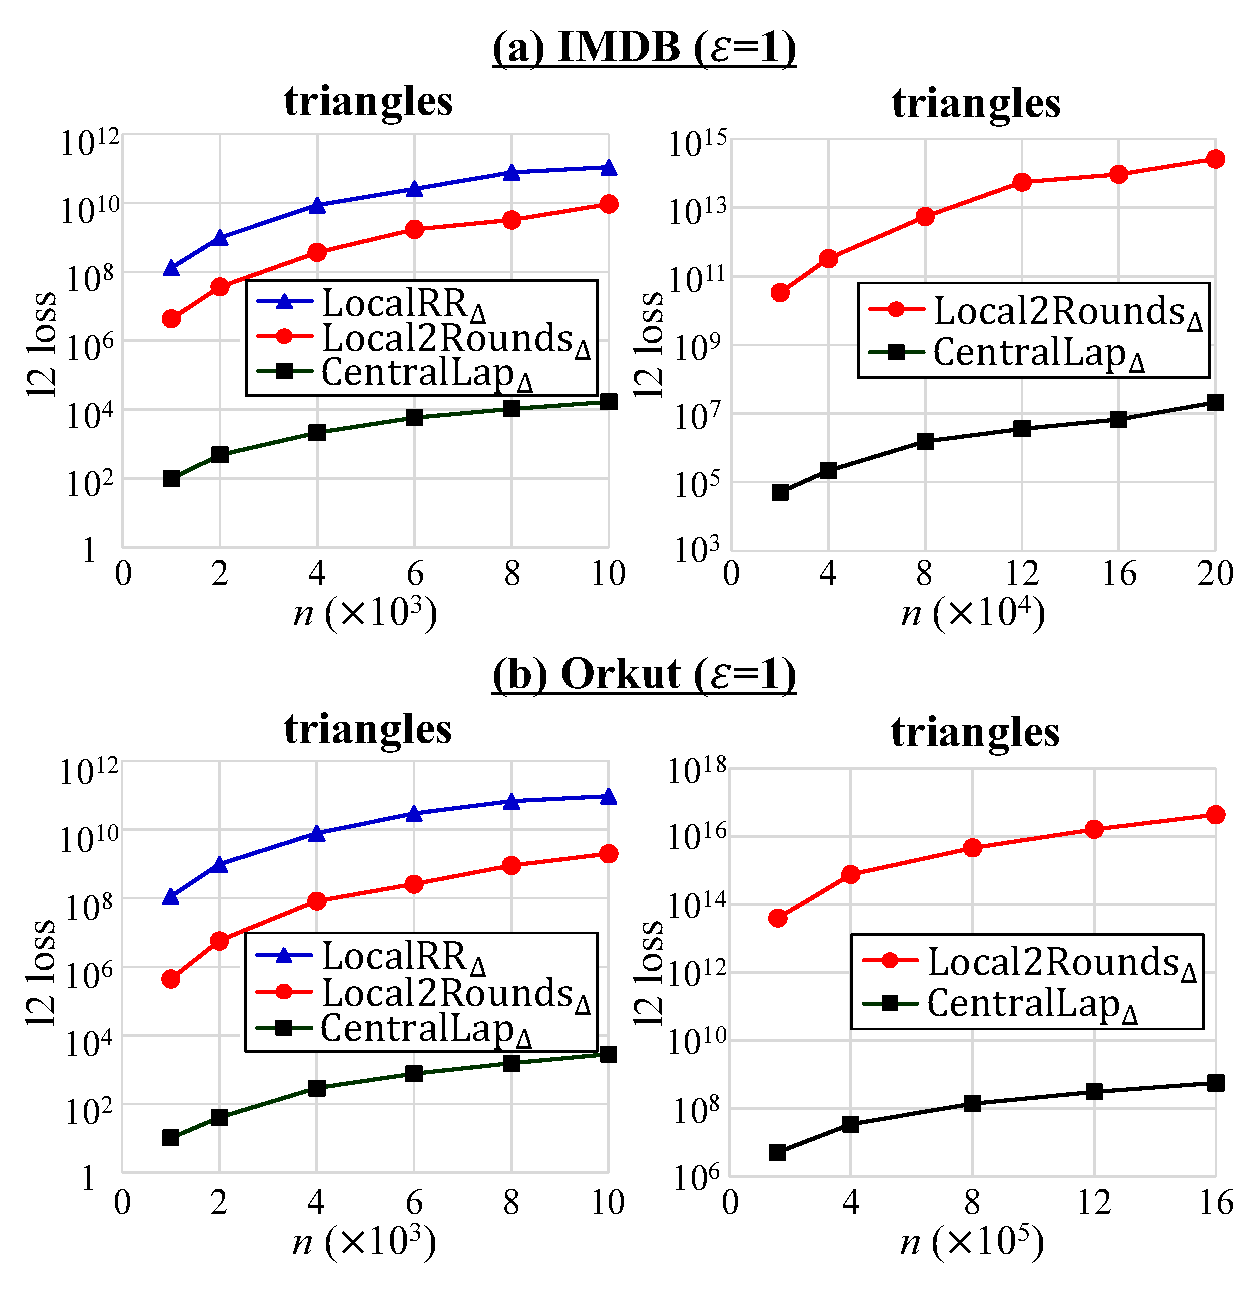
\includegraphics[width=0.99\linewidth]{fig/res1_n_l2loss_tri.pdf}
\vspace{-4mm}
\caption{Relation between the number of users $n$ and the $l_2$ loss in triangle counts when $\epsilon = 1$ ($\epsilon_1 = \epsilon_2 = \frac{1}{2}$, $\td_{max} = d_{max}$). 
Here we do not evaluate \alg{LocalRR$_\triangle$} when $n > 10000$, because it is inefficient (see Section~\ref{sub:two_rounds} ``Time complexity'').}
\label{fig:res1_n_l2loss_tri}
\end{figure}

\begin{figure}[t]
\centering
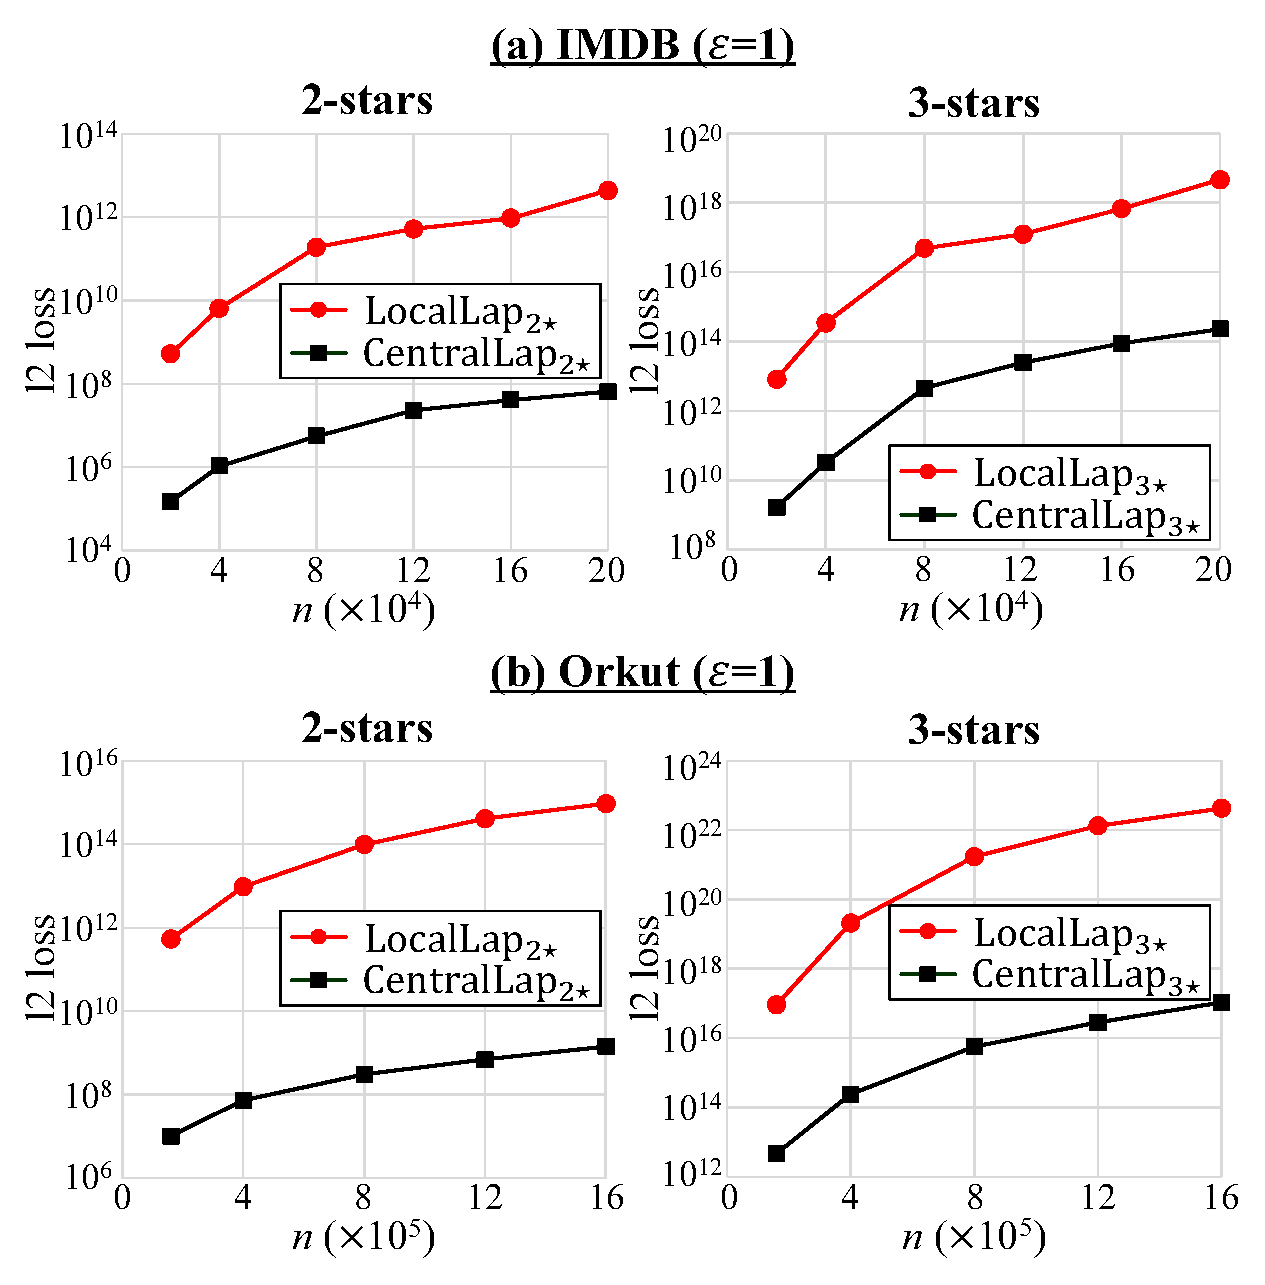
\includegraphics[width=0.99\linewidth]{fig/res1_n_l2loss_kst.pdf}
\vspace{-5mm}
\caption{Relation between the number of users $n$ and the $l_2$ loss in $k$-star counts when $\epsilon=1$ ($\epsilon_1 = \epsilon_2 = \frac{1}{2}$, $\td_{max} = d_{max}$).}
\label{fig:res1_n_l2loss_kst}
\end{figure}

\subsection{Experimental Results}
\label{sub:results}
\noindent{\textbf{Relation between $n$ and the $l_2$ loss.}}~~We first evaluated the $l_2$ loss of the estimates of 
% the numbers of triangles ($f_\triangle(G)$), $2$-stars ($f_{2\star}(G)$), and $3$-stars ($f_{3\star}(G)$), 
$f_\triangle(G)$, 
% (triangle counts), 
$f_{2\star}(G)$, 
% ($2$-star counts), 
and $f_{3\star}(G)$ 
% ($3$-star counts) 
while changing the number of users $n$. 
Figures~\ref{fig:res1_n_l2loss_tri} and \ref{fig:res1_n_l2loss_kst} shows the results ($\epsilon=1$). 
Here 
% we changed $n$ from $1000$ to $200000$ in \IMDB{}, and from $1000$ to $1600000$ in \Orkut{}. 
% Note that 
we did not evaluate \alg{LocalRR$_\triangle$} when $n$ was larger than $10000$, because \alg{LocalRR$_\triangle$} was inefficient 
% (the time complexity of \alg{LocalRR$_\triangle$} is $O(n^3)$, as described in Section~\ref{sub:two_rounds}). 
(as described in Section~\ref{sub:two_rounds} ``Time complexity''). 
% In Figures~\ref{fig:res1_n_l2loss_tri} and \ref{fig:res1_n_l2loss_kst}, 
In \alg{Local2Rounds$_\triangle$}, we set $\epsilon_1 = \epsilon_2 = \frac{1}{2}$. 
% so that $\epsilon = \epsilon_1 + \epsilon_2 = 1$. 
% In \alg{Local2Rounds$_\triangle$},  \alg{CentralLap$_\triangle$}, \alg{LocalLap$_k\star$}, and \alg{CentralLap$_k\star$}, 
As for $\td_{max}$, 
we set $\td_{max} = d_{max}$ (i.e., we assumed that $d_{max}$ is publicly available and did not perform graph projection) 
% , 
because we want to examine how well our theoretical results hold in our experiments. 
% we added the Laplacian noise with the local sensitivity in \alg{Proposal}, \alg{central (Lap)}, and \alg{local (Lap)}. 
We also evaluate the effectiveness of the private calculation of $d_{max}$ at the end of Section~\ref{sub:results}. 

Figure~\ref{fig:res1_n_l2loss_tri} shows that \alg{Local2Rounds$_\triangle$} significantly outperforms \alg{LocalRR$_\triangle$}. 
% for estimating $f_\triangle(G)$. 
Specifically, the $l_2$ loss of \alg{Local2Rounds$_\triangle$} is smaller than that of \alg{LocalRR$_\triangle$} by a factor of about $10^2$. 
% and $10^2 \sim 10^3$ in \IMDB{} and \Orkut{}, respectively. 
The difference between \alg{Local2Rounds$_\triangle$} and \alg{LocalRR$_\triangle$} is larger in \Orkut{}. 
This is because \Orkut{} is more sparse, as described in Section~\ref{sub:setup}. 
For example, when $n=10000$, the maximum degree $d_{max}$ in $G$ was $73.5$ and $27.8$ on average in \IMDB{} and \Orkut{}, respectively. 
Recall that for a fixed $\epsilon$, 
the expected $l_2$ loss of \alg{Local2Rounds$_\triangle$} and \alg{LocalRR$_\triangle$} 
can be expressed as $O(nd_{max}^3)$ and $O(n^4)$, respectively. 
Thus \alg{Local2Rounds$_\triangle$} significantly outperforms \alg{LocalRR$_\triangle$}, especially in sparse graphs. 
% datasets. 

% Figures~\ref{fig:res1_n_l2loss_tri} and \ref{fig:res1_n_l2loss_kst} show that \alg{central (Lap)} provides the best performance, which is consistent with our theoretical results; i.e., 

Figures~\ref{fig:res1_n_l2loss_tri} and \ref{fig:res1_n_l2loss_kst} show that the $l_2$ loss is roughly consistent with 
our upper-bounds in terms of $n$. 
Specifically, 
\alg{LocalRR$_\triangle$}, 
\alg{Local2Rounds$_\triangle$},  \alg{CentralLap$_\triangle$}, 
\alg{LocalLap$_{k\star}$}, and 
\alg{CentralLap$_{k\star}$} achieve 
the expected $l_2$ loss of $O(n^4)$, $O(nd_{max}^3)$, $O(d_{max}^2)$, $O(nd_{max}^{2k-2})$, and $O(d_{max}^{2k-2})$, respectively. 
Here note that 
% the maximum degree $d_{max}$ increases roughly in proportion to $n$ (though $d_{max}$ is much smaller than $n$), 
each user's degree increases roughly in proportion to $n$ (though the degree is much smaller than $n$), 
as we randomly select $n$ users from the whole graph $G^*$. Assuming that $d_{max} = O(n)$,  Figures~\ref{fig:res1_n_l2loss_tri} and \ref{fig:res1_n_l2loss_kst} are roughly consistent with the upper-bounds. 
The figures also show the limitations of the local model in terms of the utility when compared to the centralized model.

% when we increase $n$ by a factor of $10$, 
% the $l_2$ loss in triangle counts increases by a factor of about $10^4$, $10^4$, $10^2$ in \alg{LocalRR$_\triangle$}, \alg{Local2Rounds$_\triangle$}, and \alg{central (Lap)}, respectively. 
% Therefore, the experimental results are roughly consistent with our theoretical results that the expected $l_2$ loss of \alg{LocalRR$_\triangle$}, \alg{Local2Rounds$_\triangle$}, and \alg{CentralLap$_\triangle$} is $O(n^4)$, $O(nd_{max}^3)$, and $O(d_{max}^2)$, respectively. 
% The same applies to $k$-star counts. 

\smallskip
\noindent{\textbf{Relation between $\epsilon$ and the $l_2$ loss.}}~~Next we evaluated the $l_2$ loss 
% of the estimates of $f_\triangle(G)$ (triangle counts) and $f_{2\star}(G)$ ($2$-star counts), 
when we changed the privacy budget $\epsilon$ in edge LDP. 
Figure~\ref{fig:res2_eps_l2loss} shows the results for triangles and $2$-stars ($n=10000$). 
% (the result of $3$-stars is similar to that of $2$-stars, and therefore we omit the result of $3$-stars). 
Here we omit the result of $3$-stars because it is similar to that of $2$-stars. 
In \alg{Local2Rounds$_\triangle$}, we set $\epsilon_1 = \epsilon_2 = \frac{\epsilon}{2}$. 

Figure~\ref{fig:res2_eps_l2loss} shows that the $l_2$ loss is roughly consistent with 
% the expected $l_2$ loss in 
% our theoretical analysis 
our upper-bounds in terms of $\epsilon$. 
For example, when we decrease $\epsilon$ from $0.4$ to $0.1$, the $l_2$ loss 
% in triangle counts 
increases by a factor of about $5000$, $200$, and $16$ for both the datasets in \alg{LocalRR$_\triangle$}, \alg{Local2Rounds$_\triangle$}, and \alg{CentralLap$_\triangle$}, respectively. 
% This is 
They are 
roughly consistent with our theoretical results 
that for small $\epsilon$, the expected $l_2$ loss of \alg{LocalRR$_\triangle$}, \alg{Local2Rounds$_\triangle$}, and \alg{CentralLap$_\triangle$} is  $O(\epsilon^{-6})$\footnote{We used $e^\epsilon \approx \epsilon + 1$ to derive the upper-bound of \alg{LocalRR$_\triangle$} for small $\epsilon$.}, $O(\epsilon^{-4})$, and $O(\epsilon^{-2})$, respectively. 
% The same applies to large $\epsilon$ (e.g., $\epsilon = 1$ or $2$). 

\begin{figure}[t]
\centering
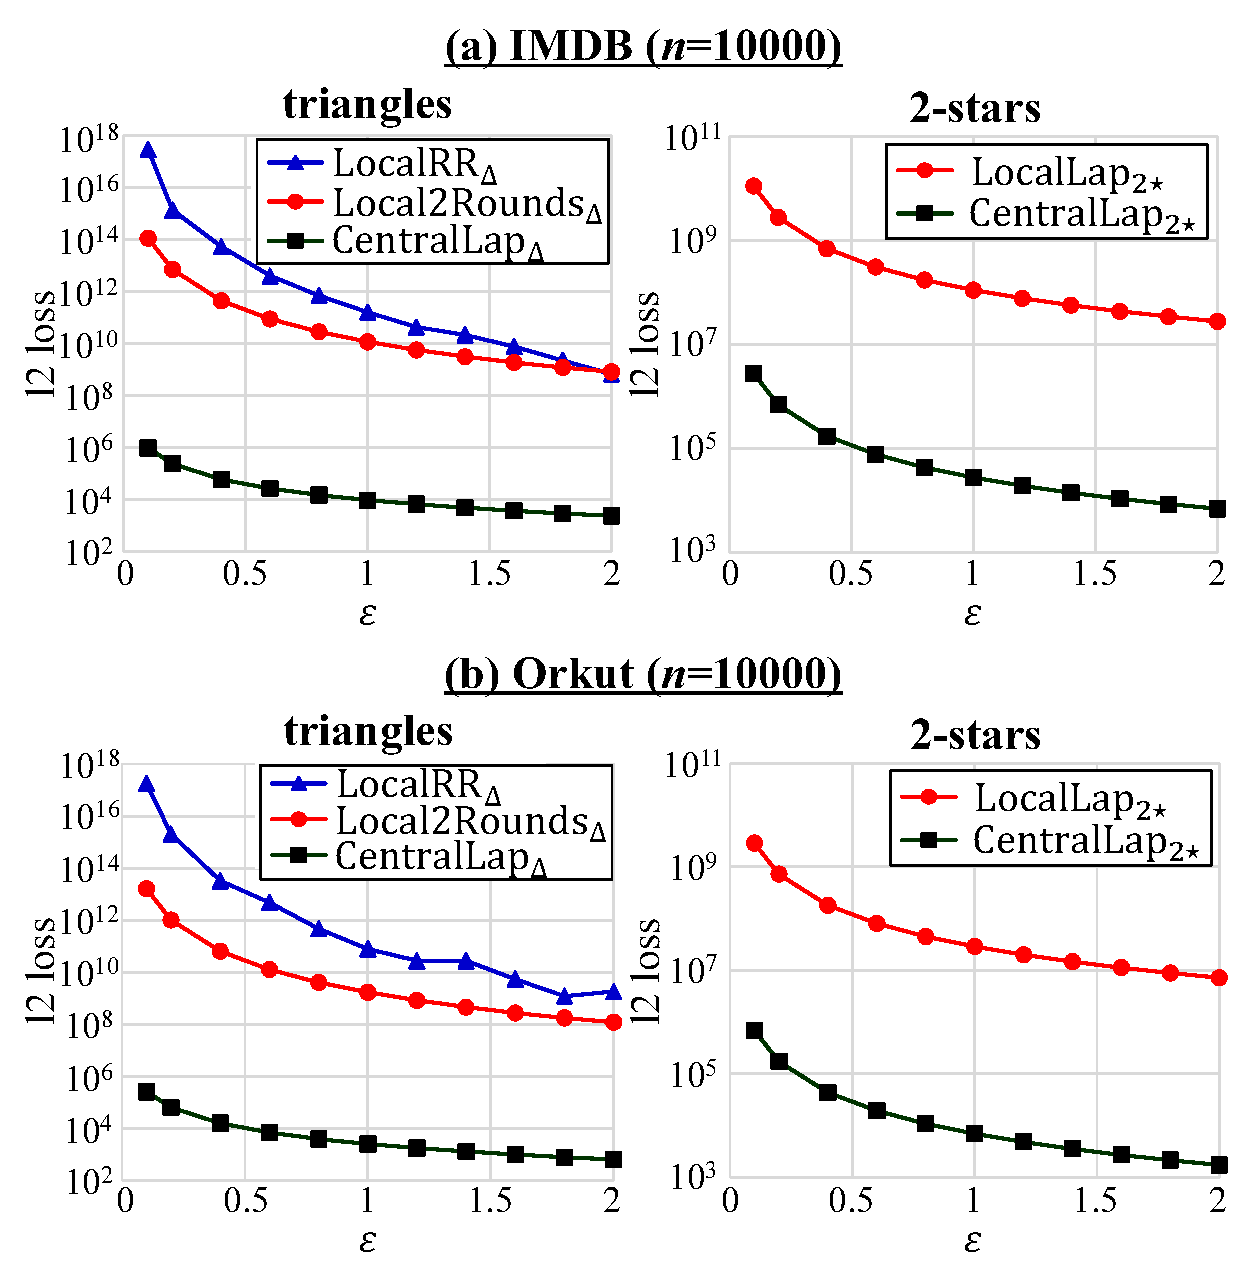
\includegraphics[width=0.99\linewidth]{fig/res2_eps_l2loss.pdf}
\vspace{-5mm}
\caption{Relation between $\epsilon$ in edge LDP and the $l_2$ loss when $n=10000$ ($\epsilon_1 = \epsilon_2 = \frac{\epsilon}{2}$, $\td_{max} = d_{max}$).}
\label{fig:res2_eps_l2loss}
\end{figure}

\begin{figure}[t]
\centering
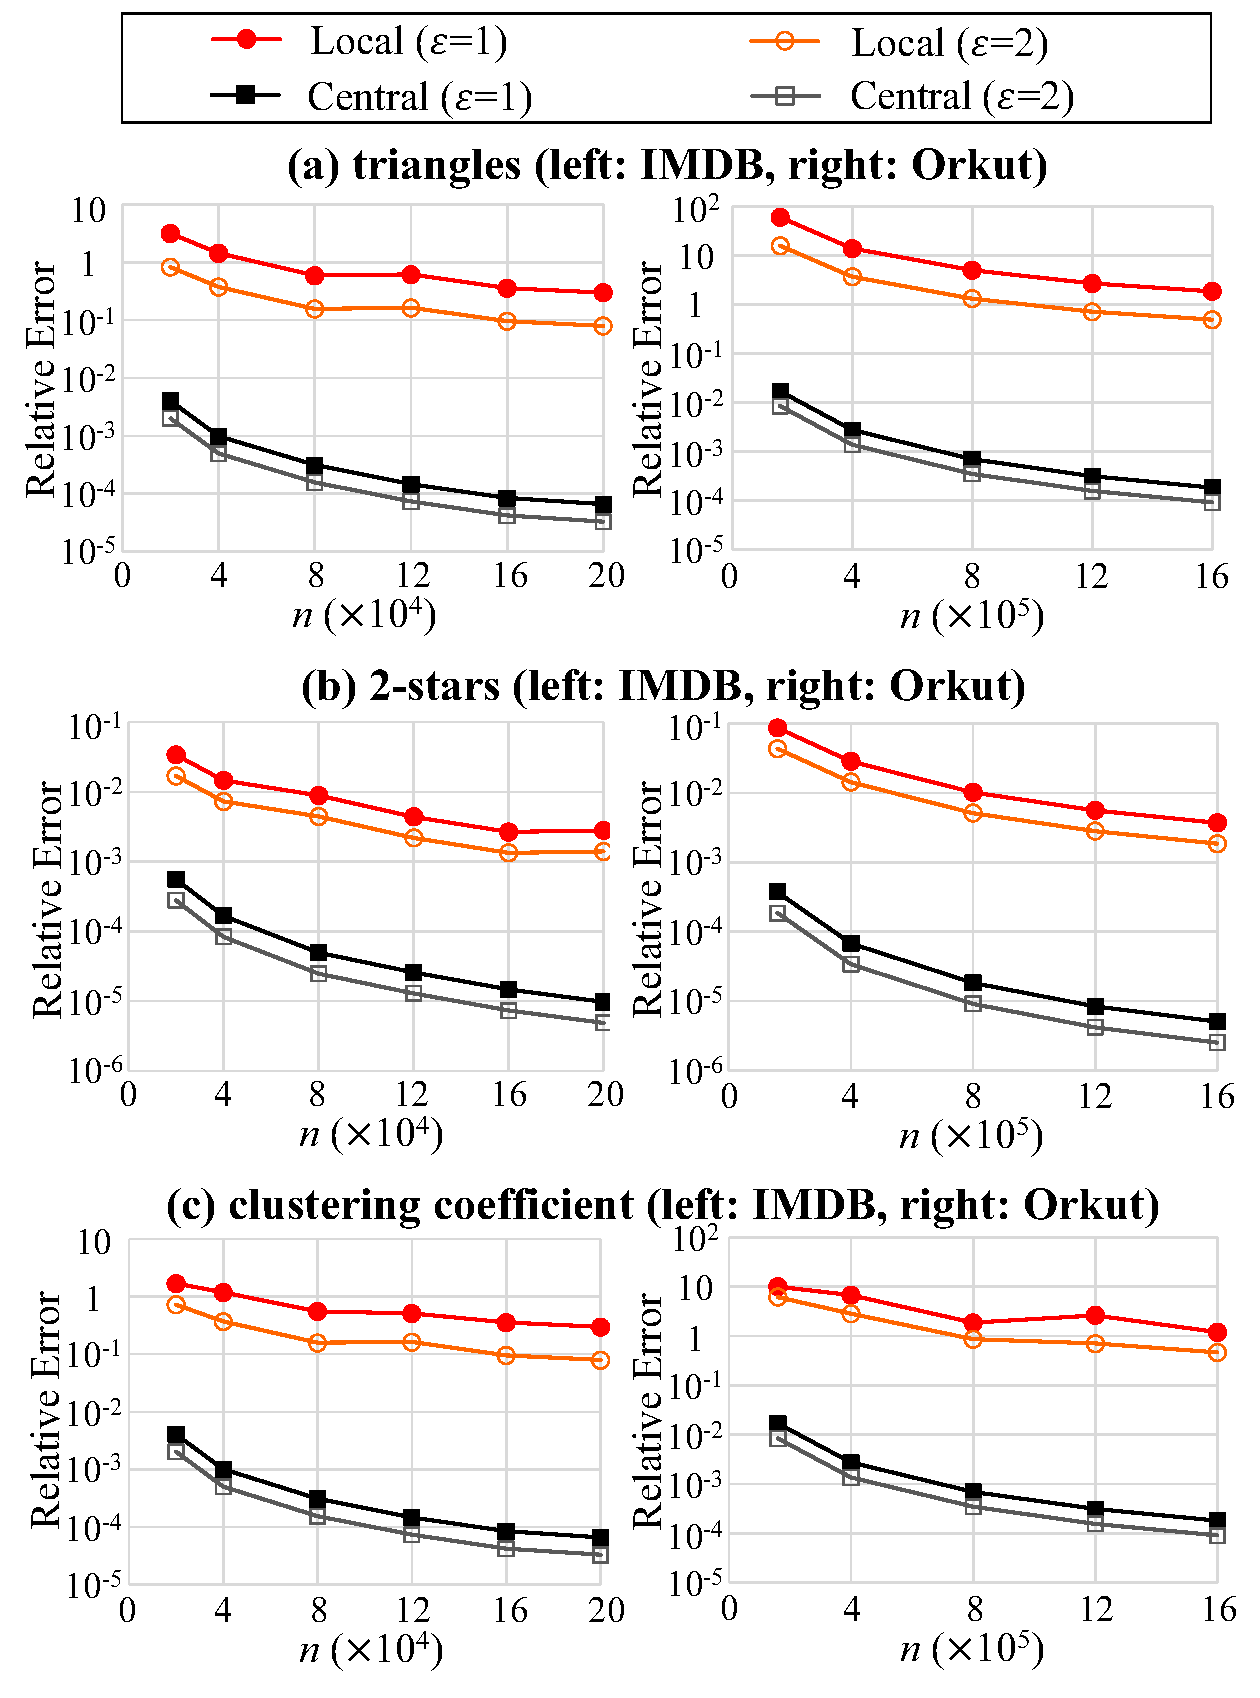
\includegraphics[width=0.99\linewidth]{fig/res3_n_relerr.pdf}
\vspace{-5mm}
\caption{Relation between 
% the number of users 
$n$ and the relative error. In the local model, we used \alg{Local2Rounds$_\triangle$} ($\epsilon = 1$ or $2$) and \alg{LocalLap$_k\star$} ($\epsilon = 1$ or $2$) for estimating triangle counts $f_\triangle(G)$ and $k$-star counts $f_{k\star}(G)$, respectively ($\td_{max} = d_{max}$).}
\label{fig:res3_n_relerr}
\end{figure}

Figure~\ref{fig:res2_eps_l2loss} also shows that 
\alg{Local2Rounds$_\triangle$} significantly outperforms \alg{LocalRR$_\triangle$} especially when $\epsilon$ is small, which is also consistent with our theoretical results. 
Conversely, the difference between \alg{LocalRR$_\triangle$} and \alg{Local2Rounds$_\triangle$} is small when $\epsilon$ is large. 
This is because when $\epsilon$ is large, the RR outputs the true value with high probability. 
For example, when 
% $\epsilon \geq 3$, 
$\epsilon \geq 5$, 
the RR outputs the true value with 
% $\frac{e^\epsilon}{e^\epsilon+1} > 0.95$. 
$\frac{e^\epsilon}{e^\epsilon+1} > 0.993$. 
% We also confirmed that when $\epsilon \geq 3$, the $l_2$ loss of \alg{LocalRR$_\triangle$} is smaller than \alg{Local2Rounds$_\triangle$} in both the datasets. 
However, \alg{LocalRR$_\triangle$} with 
% $\epsilon \geq 3$ 
such a large value of $\epsilon$ 
does not guarantee strong privacy, because it outputs the true value in most cases. 
% with more than $95\%$. 
\alg{Local2Rounds$_\triangle$} significantly outperforms \alg{LocalRR$_\triangle$} 
% for a reasonable range of $\epsilon$. 
when we want to estimate $f_\triangle(G)$ or $f_{k\star}(G)$ 
with a strong privacy guarantee; e.g., $\epsilon \leq 1$ \cite{DP_Li}. 

\smallskip
\noindent{\textbf{Relative error.}}~~As the number of users $n$ increases, the numbers of triangles $f_\triangle(G)$ and $k$-stars $f_{k\star}(G)$ increase. 
% , and this 
This causes the increase of the $l_2$ loss. 
Therefore, we also evaluated the relative error, as described in Section~\ref{sub:graph_statistics}. 

Figure~\ref{fig:res3_n_relerr} shows the relation between $n$ and the relative error 
(we omit the result of $3$-stars because it is similar to that of $2$-stars). 
In the local model, we used \alg{Local2Rounds$_\triangle$} and \alg{LocalLap$_k\star$} for estimating 
% triangle counts 
$f_\triangle(G)$ 
and 
% $k$-star counts, 
$f_{k\star}(G)$, 
respectively 
(we did not use \alg{Local2RR$_\triangle$}, because it is both inaccurate and inefficient). 
For both algorithms, we set $\epsilon = 1$ or $2$ 
($\epsilon_1 = \epsilon_2 = \frac{\epsilon}{2}$ in \alg{Local2Rounds$_\triangle$}) and $\td_{max} = d_{max}$. 
Then we estimated the clustering coefficient as: $\frac{3\hf_{\triangle}(G, \epsilon_1, \epsilon_2, d_{max})}{\hf_{k\star}(G, \epsilon, d_{max})}$, where 
$\hf_{\triangle}(G, \epsilon_1, \epsilon_2, d_{max})$ and 
$\hf_{k\star}(G, \epsilon, d_{max})$ are the estimates of $f_\triangle(G)$ and $f_{k\star}(G)$, respectively. 
If the estimate of the clustering coefficient is smaller than $0$ (resp.~larger than $1$), we set the estimate to $0$ (resp.~$1$) because the clustering coefficient is always between $0$ and $1$. 
In the centralized model, we used \alg{CentralLap$_\triangle$} and \alg{CentralLap$_k\star$} ($\epsilon=1$ or $2$, $\td_{max} = d_{max}$) and calculated the clustering coefficient in the same way. 

Figure~\ref{fig:res3_n_relerr} shows that for all cases, the relative error decreases with increase in $n$. 
This is because both $f_\triangle(G)$ and $f_{k\star}(G)$ significantly increase with increase in $n$. 
Specifically, let $f_{\triangle,v_i}(G) \in \nnints$ the number of triangles that involve user $v_i$, and $f_{k\star,v_i}(G) \in \nnints$ be the number of $k$-stars of which user $v_i$ is a center. 
Then $f_\triangle(G) = \frac{1}{3}\sum_{i=1}^n f_{\triangle,v_i}(G)$ and $f_{k\star,v_i}(G) = \sum_{i=1}^n f_{k\star,v_i}(G)$. 
Since both $f_{\triangle,v_i}(G)$ and $f_{k\star,v_i}(G)$ increase with increase in $n$, both $f_\triangle(G)$ and $f_{k\star}(G)$ increase \textit{at least} in proportion to $n$. 
Thus $f_\triangle(G)^2 \geq \Omega(n^2)$ and $f_{k\star}(G)^2 \geq \Omega(n^2)$. 
In contrast, \alg{Local2Rounds$_\triangle$}, \alg{LocalLap$_k\star$}, \alg{CentralLap$_\triangle$}, and \alg{CentralLap$_k\star$} achieve the expected $l_2$ loss of $O(n)$, $O(n)$, $O(1)$, and $O(1)$, respectively (when we ignore $d_{max}$ and $\epsilon$), all of which are smaller than $O(n^2)$. 
% the value $\frac{|\hf(G) - f(G)|}{|f(G)|}$ decreases with increase in $n$. 
% This explains the reason that 
Therefore, the relative error decreases with increase in $n$. 

This result demonstrates that we can accurately estimate graph statistics for large $n$ in the local model. 
In particular, the relative error is smaller in \IMDB{} 
% , 
because \IMDB{} is denser and includes a larger number of triangles and $k$-stars; i.e., the denominator of the relative error is large. 
For example, when $n=200000$ and $\epsilon=1$, the relative error is 
% $0.19$, 
$0.30$ and 
$0.0028$ 
% , and $0.015$ 
for triangles and $2$-stars, 
% , and $3$-stars, 
respectively. 
Note that the clustering coefficient requires $2\epsilon$ 
% , 
because we need to estimate both $f_\triangle(G)$ and $f_{k\star}(G)$. 
Yet, we can still accurately calculate the clustering coefficient with a moderate privacy budget; 
% $\epsilon$; 
e.g., the relative error of the clustering coefficient is 
%$0.19$ 
$0.30$ 
when the privacy budget is $2$ (i.e., $\epsilon = 1$).
If $n$ is larger, then $\epsilon$ would be smaller at the same value of the relative error. 

\begin{figure}[t]
\centering
% 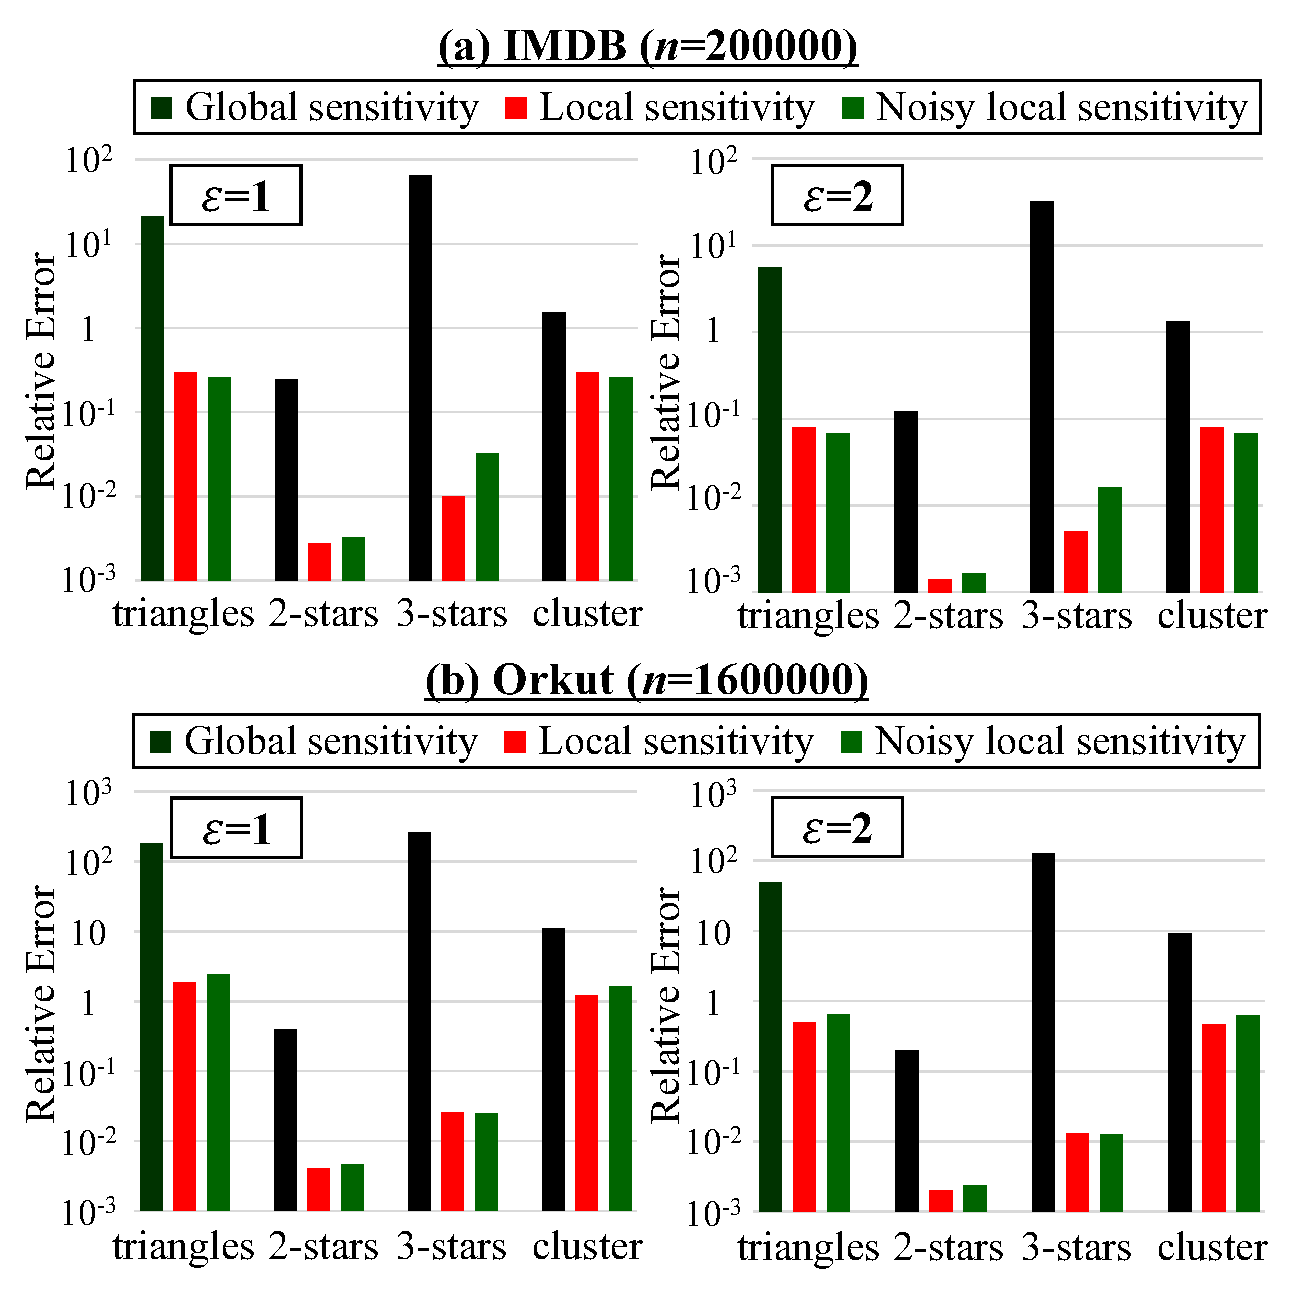
\includegraphics[width=0.99\linewidth]{fig/res4_noisy_local.pdf}
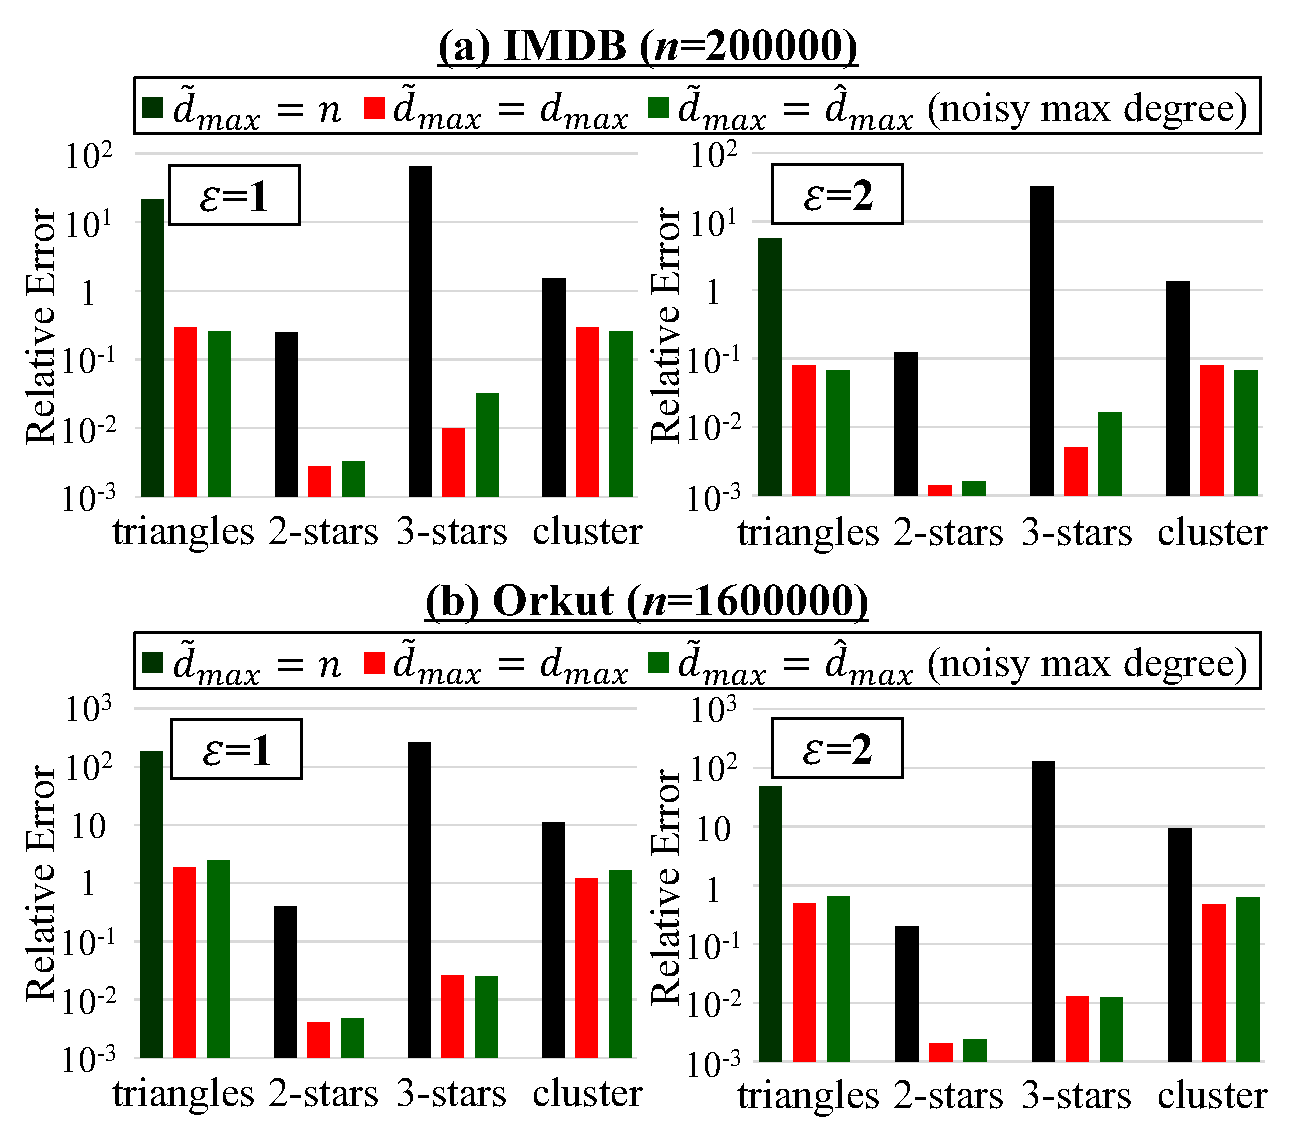
\includegraphics[width=0.99\linewidth]{fig/res4_noisy_max.pdf}
\vspace{-4mm}
\caption{Relative error 
% for 
% three types of sensitivity: 
% global sensitivity ($\td_{max} = n$), 
% local sensitivity ($\td_{max} = d_{max}$), and 
% noisy local sensitivity ($\td_{max} = \hd_{max}$). 
when $\td_{max} = n$ (\#users), 
$d_{max}$ (max degree), or 
$\hd_{max}$ (noisy max degree). 
% $\hd_{max}$ represents the private estimate of $d_{max}$; i.e., noisy max degree. 
We used \alg{Local2Rounds$_\triangle$} ($\epsilon = 1$ or $2$) and \alg{LocalLap$_k\star$} ($\epsilon = 1$ or $2$) for estimating triangle counts $f_\triangle(G)$ and $k$-star counts $f_{k\star}(G)$, respectively. 
% In ``Local sensitivity (Cauchy),'' we added the Cauchy noise (rather than the Laplacian noise) with the local sensitivity, which is always smaller than or equal to the smooth sensitivity \cite{Karwa_PVLDB11}.
}
\label{fig:res4_noisy_local}
\end{figure}

\smallskip
\noindent{\textbf{Private calculation of $d_{max}$.}}~~We have so far assumed that $\td_{max} = d_{max}$ (i.e., $d_{max}$ is publicly available) in our experiments. 
% However, it is difficult for the users and the data collector to know the exact value of $d_{max}$ in advance. 
% Therefore, we 
We 
finally evaluate the methods to privately calculate $d_{max}$ with $\epsilon_0$-edge LDP 
% , which are 
(described in Sections~\ref{sub:non-interactive_k_stars} and \ref{sub:two_rounds}). 
% show that even if we privately calculate $d_{max}$ with edge LDP, we can accurately estimate graph statistics in the local model. 

Specifically, we used \alg{Local2Rounds$_\triangle$} and \alg{LocalLap$_k\star$} for estimating $f_\triangle(G)$ and $f_{k\star}(G)$, respectively, and evaluated the following three methods for setting $\td_{max}$: 
% the sensitivity: 
% \begin{enumerate}
%     \item Set $\td_{max} = n$. We call this method the \textit{global sensitivity method} because it results in adding the Laplacian noise with the global sensitivity in Definition~\ref{def:global_sen}.
%     \item Set $\td_{max} = d_{max}$. We call this method the \textit{local sensitivity method} because it results in adding the Laplacian noise with the local sensitivity. 
% \end{enumerate}
(i) 
% set 
$\td_{max} = n$; 
(ii) 
% set 
$\td_{max} = d_{max}$; 
(iii) 
% set 
$\td_{max} = \hd_{max}$, where $\hd_{max}$ is the private estimate of $d_{max}$ 
% (i.e., 
(noisy max degree) in Sections~\ref{sub:non-interactive_k_stars} and \ref{sub:two_rounds}. 
% Note that the first (resp.~second) method results in adding the Laplacian noise with the global (resp.~local) sensitivity without using graph projection. 
% Therefore, we refer to the first method (i) as the \textit{global sensitivity method}, the second method (ii) as the \textit{local sensitivity method}, and the third method (iii) as the \textit{noisy local sensitivity method}. 

We set $n=200000$ in \IMDB{} and $n=1600000$ in \Orkut{}. 
Regarding the total privacy budget $\epsilon$ in edge LDP for estimating $f_\triangle(G)$ or $f_{k\star}(G)$, we set $\epsilon=1$ or $2$. 
We used $\frac{\epsilon}{10}$ for privately calculating $d_{max}$ (i.e., $\epsilon_0 = \frac{\epsilon}{10}$), and the remaining privacy budget $\frac{9\epsilon}{10}$ as input to \alg{Local2Rounds$_\triangle$} or \alg{LocalLap$_k\star$}. 
% estimating $f_\triangle(G)$ or $f_{k\star}(G)$. 
In \alg{Local2Rounds$_\triangle$}, we set $\epsilon_1 = \epsilon_2$; i.e., we set $(\epsilon_0, \epsilon_1, \epsilon_2) = (0.1, 0.45, 0.45)$ or $(0.2, 0.9, 0.9)$. 
% For example, \alg{Local2Rounds$_\triangle$} with $(\epsilon_0, \epsilon_1, \epsilon_2) = (0.1, 0.45, 0.45)$ provides $1$-edge LDP and $1.1$-entire edge LDP (see Section~\ref{sub:two_rounds}). 
Then we estimated the clustering coefficient in the same way as Figure~\ref{fig:res3_n_relerr}. 

Figure~\ref{fig:res4_noisy_local} shows the results. 
Figure~\ref{fig:res4_noisy_local} shows that 
% the noisy local sensitivity method 
the algorithms with $\td_{max} = \hd_{max}$ (noisy max degree) 
achieves the relative error close to (sometimes almost the same as) 
% the local sensitivity method, 
the algorithms with $\td_{max} = d_{max}$ 
and significantly outperforms 
% the global sensitivity method. 
the algorithms with $\td_{max} = n$. 
This means that we can privately estimate $d_{max}$ without a significant loss of utility. 
% Recall that the private calculation of $d_{max}$ does not increase the number of rounds in \alg{Local2Rounds$_\triangle$}. 
% Therefore, we can privately estimate $d_{max}$ and then accurately estimate all the graph statistics (i.e., triangles, $k$-stars, and the clustering coefficient) within two rounds.

\smallskip
\noindent{\textbf{Summary of results.}}~~In summary, 
% our experimental results were roughly consistent with our theoretical results. 
our experimental results showed that the estimation error of triangle counts is significantly reduced by introducing the interaction between users and a data collector. 
The results also showed that 
% we can accurately estimate graph statistics in the local model. 
% In particular, 
we can achieve small relative errors 
(much smaller than 1) for subgraph counts 
% for a large number of users $n$ 
with privacy budget $\epsilon=1$ or $2$ in edge LDP. 
% The results also showed that we can privately estimate the maximum degree $d_{max}$, which is required in both \alg{Local2Rounds$_\triangle$} and \alg{LocalLap$_k\star$}, without a significant loss of utility. 

As described in Section~\ref{sec:intro}, non-private 
% triangle or $k$-star 
subgraph 
counts may reveal some friendship information, and a central server may face data breaches. 
Our LDP algorithms are highly beneficial because they enable us to analyze the connection patterns in a graph 
(i.e., subgraph counts) 
or to understand how likely two friends of an individual will also be a friend 
% (which is useful for friend suggestion) 
(i.e., clustering coefficient) 
while strongly protecting individual privacy.


\section{Conclusions}
\label{sec:conclusions}
% In this paper, 
We presented a series of algorithms for counting triangles and $k$-stars under LDP. 
We 
% analyzed the upper-bounds on the expected $l_2$ loss for these algorithms, and 
showed that an additional round can significantly reduce the estimation error in triangles, and the algorithm based on the Laplacian mechanism provides an order optimal error in the non-interactive local model. 
We also showed lower-bounds for general functions including triangles and $k$-stars. 
We conducted experiments using two real datasets, and showed that our algorithms achieve small relative errors, especially when the number of users is large.

As future work, we would like to develop algorithms for other subgraph counts such as cliques and $k$-triangles \cite{Karwa_PVLDB11}. 

% %-------------------------------------------------------------------------------
\section*{Acknowledgments}
Kamalika Chaudhuri and Jacob Imola would like to thank ONR under N00014-20-1-2334 and UC Lab Fees under LFR 18-548554  for research support. 
Takao Murakami was supported in part by JSPS KAKENHI JP19H04113.


